\chapter{シミュレーション最適化 }
\label{chap::sim}

\hspace{1zw}この章ではビル全体の空調設定スケジュールを最適化するために,ビルシミュレータを用いる手段について述べる.

\section{概要}
最適化システムの構成を\figref{fig::sim_system}に示す.\figref{fig::math_system}の評価部における数理モデルの代替として,ビルシミュレータEnergyPlus \cite{NREL19}を用いる.EnergyPlusは,米国エネルギー省再生可能エネルギー研究所(NREL)が開発した建築物のエネルギーシミュレータであり,建物内外の熱移動とそれに伴う温湿度変化,空調,換気,照明等各設備のエネルギー消費量を算出できる.EnergyPlusは,ビル躯体の構造・設備・エネルギー使用設定等の建物情報,外気温・外気湿度・天候・日射量などの気象情報,空調設定温度スケジュール情報を入力することで,エネルギー消費量や各部屋の環境および快適性の時系列データを算出できる.\chapref{chap::math}における数理モデルをEnergyPlusによるシミュレーションで代替することで,部屋単位の詳細な数理モデルの構築を回避する.EnergyPlusシミュレータでシミュレーションを行うためには,シミュレータにシミュレーション対象のビルモデルを入力する必要がある.本論文では,建築用のモデリングソフトウエアRevitを用いて,ビルの構造,設備,エネルギー設定等を含むオフィスビルのモデルを構築する.

\begin{figure*}[t]
  \begin{center}
    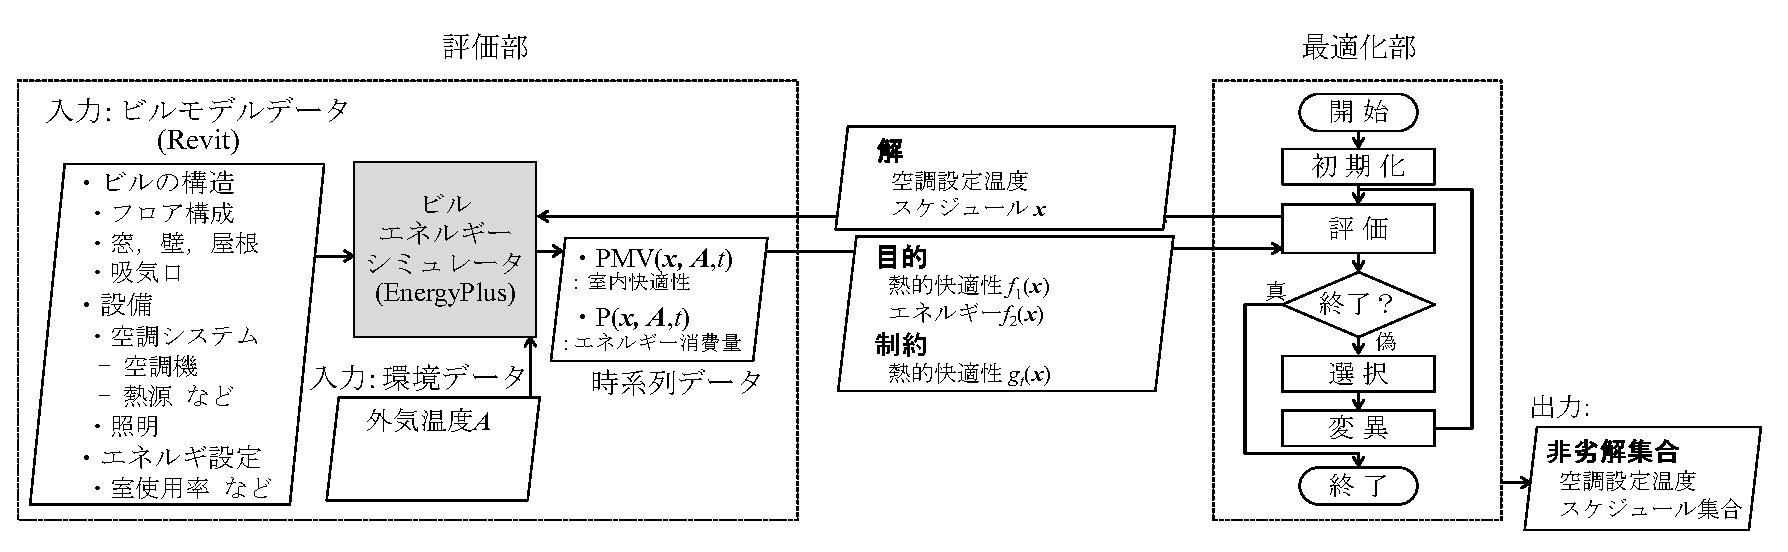
\includegraphics[width=1.1\linewidth]{fig/sim_system.eps}
  \end{center}
  \caption{シミュレーション最適化システム}
  \label{fig::sim_system}
\end{figure*}


\section{シミュレーション最適化における解評価}\label{sec::sim_model}
\subsection{ビルのモデルとシミュレーション}
本章の最適化対象は,オフィスの一室ではなく,ビル全体である.本研究で作成したシミュレーション対象のオフィスビルのモデルを\figref{fig::sim_office_building}に示す.また,主な諸元を\tabref{tab::sim_description}に,1階のフロアレイアウト\figref{fig::sim_groundfloor}に,基準階のフロアレイアウトを\figref{fig::sim_typicalfloor}に示す.このビルは,地上8階建てで,延床面積が11,781$[m^2]$であり,全フロアにオフィスを持つ.ビル内のオフィス数は54,室内快適性とエネルギー消費量の解析対象にする空間数は,廊下,トイレ,エレベータホールなども含めて114とした.また,エネルギー解析のための設定を\tabref{tab::sim_analysis_param}に示す.本ビルにはセントラル空調システムが導入されており,冷温水を用いて各フロアの空調機が冷風と温風を作り,可変風量ユニットを経由して各部屋に供給する.

\begin{figure}[htbp]
  \begin{center}
    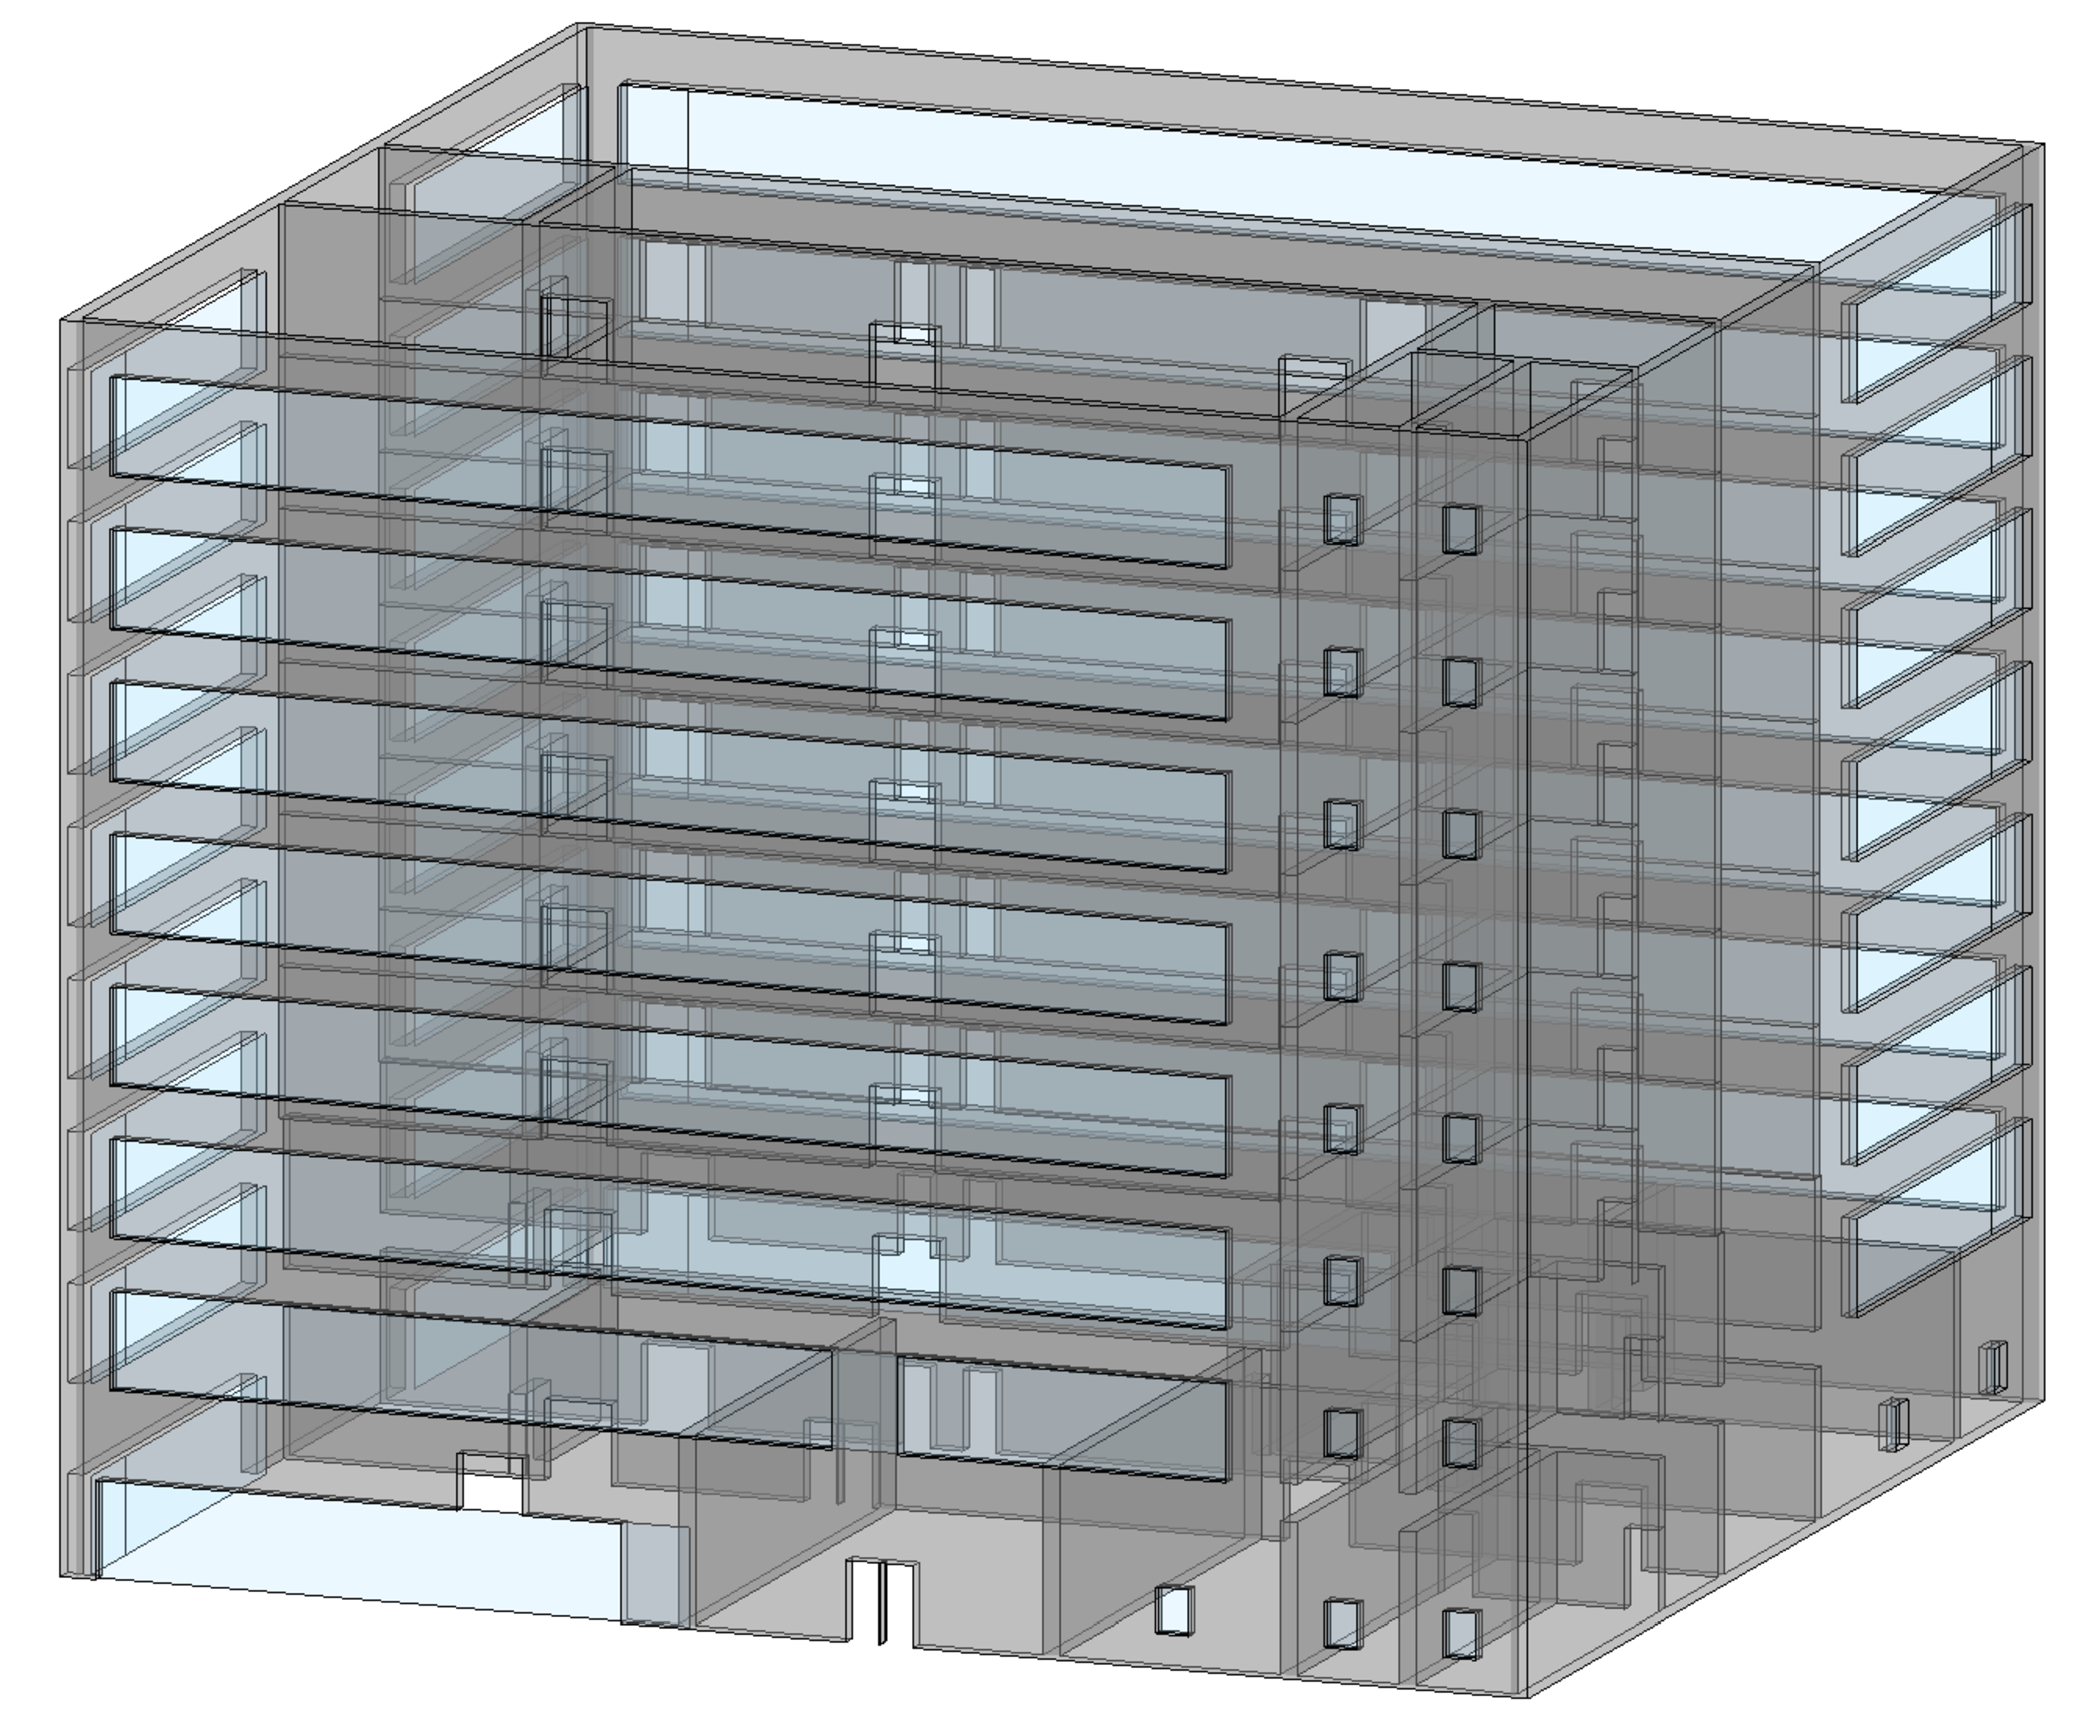
\includegraphics[width=0.6\linewidth]{fig/sim_office_building.eps}
  \end{center}
  \caption{最適化対象のオフィスビルモデルの外観}
  \label{fig::sim_office_building}
\end{figure}

\begin{table}[htbp]
  {\small
    \begin{center}
      \caption{最適化対象のオフィスビルの主要諸元}
      \label{tab::sim_description}
      \begin{tabular}{c|cccc}
        \hline
        項目     & 値                 \\
        \hline \hline
        建物用途 & オフィスビル       \\
        構造     & 鉄筋コンクリート造 \\
        敷地面積 & 5,000 [m$^2$]      \\
        建築面積 & 1,508 [m$^2$]      \\
        延床面積 & 11,781 [m$^2$]     \\
        階数     & 8                  \\
        \hline
      \end{tabular}
    \end{center}
  }
\end{table}

\begin{figure}[htbp]
  \begin{center}
    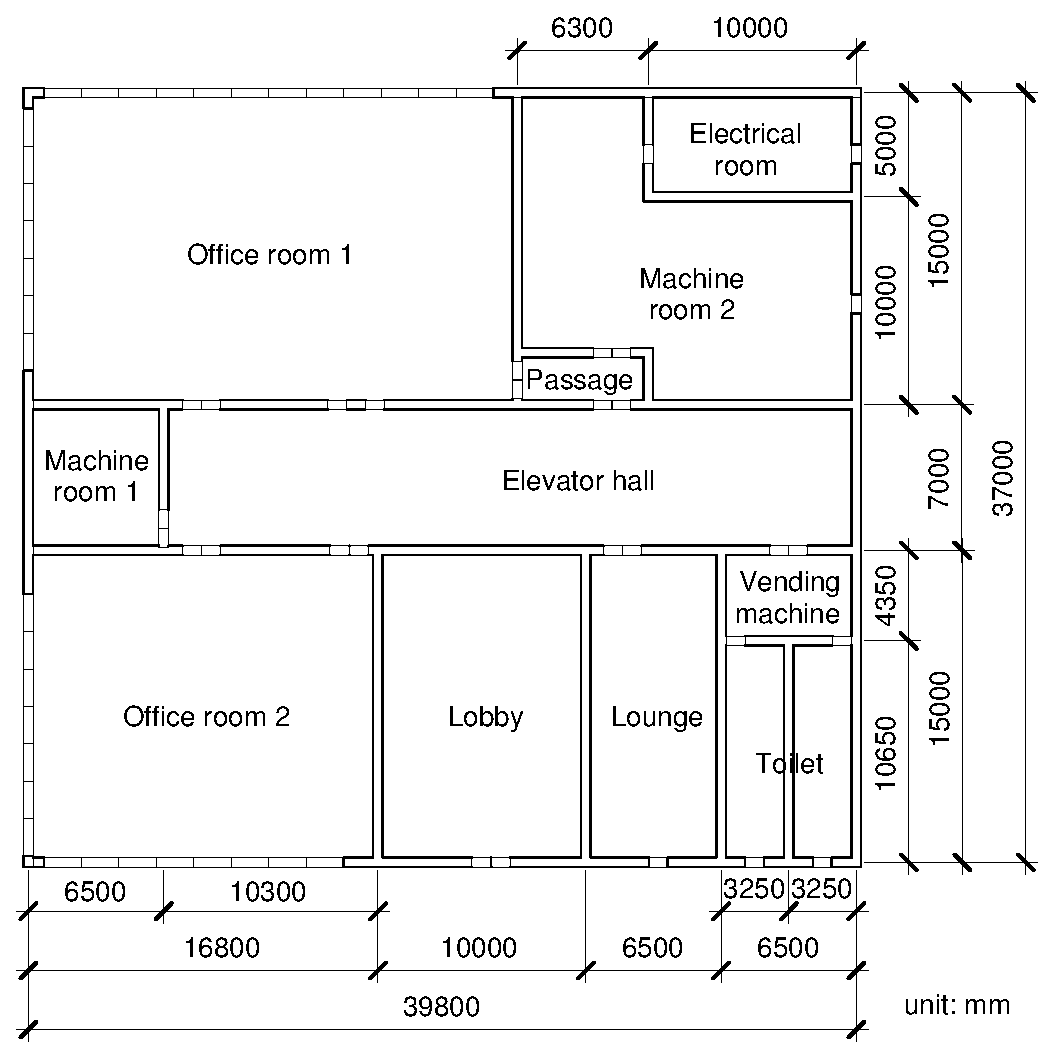
\includegraphics[width=0.65\linewidth]{fig/sim_groundfloor_en.eps}
  \end{center}
  \caption{1階のフロアレイアウト}
  \label{fig::sim_groundfloor}
\end{figure}
\begin{figure}[ht]
  \begin{center}
    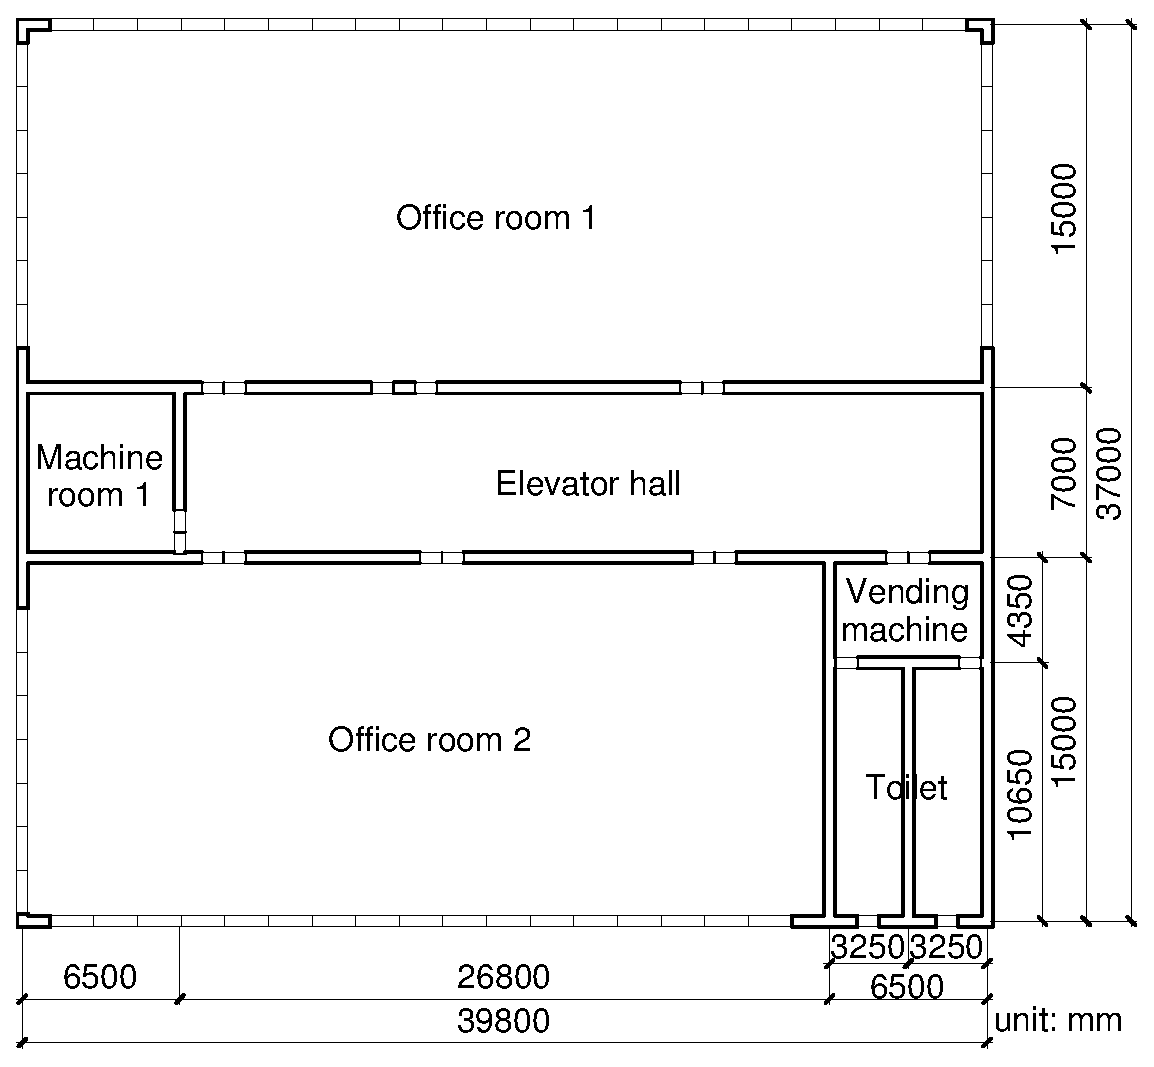
\includegraphics[width=0.65\linewidth]{fig/sim_typicalfloor_en.eps}
  \end{center}
  \caption{基準階のフロアレイアウト}
  \label{fig::sim_typicalfloor}
\end{figure}


\begin{table}[htbp]
  {\small
    \begin{center}
      \caption{エネルギー解析設定}
      \label{tab::sim_analysis_param}
      \begin{tabular}{c|cccc}
        \hline
        設定項目                     & 値                                      \\
        \hline \hline
        \raisebox{2mm}{外壁断熱材}   & \shortstack{発泡ポリスチレンフォーム    \\ (R値 \footnotemark[1] = 1.73 [m$^2$ K/W]) }\\
        \raisebox{2mm}{屋根断熱材}   & \shortstack{発泡ポリスチレンフォーム    \\ (R値 = 3.87 [m$^2$ K/W]) }\\
        \raisebox{2mm}{窓}           & \shortstack{Low-Eペアガラス             \\ (低日射熱取得率タイプ)}\\
        \raisebox{5mm}{空調システム} & \shortstack{中央熱源方式                \\冷温水機(COP \footnotemark[2]=5.96) \\ 可変風量システム}\\
        外気導入量                   & 1.38 [$ LPS$ \footnotemark[3]$ / m^2 $] \\
        人体発熱量                   & 顕熱: 55 ,  潜熱: 64 [W/人]             \\
        \shortstack{執務者の                                                   \\占有面積} & \raisebox{2mm}{10 [m$^2$/人]} \\
        照明発熱量                   & 10.6 [W/m$^2$]                          \\
        電気機器発熱量               & 12 [W/m$^2$]                            \\
        \hline
      \end{tabular}
    \end{center}
  }
\end{table}

\subsection{設計変数}
本章では,\chapref{chap::math}と同様に,空調設定温度スケジュール$t_{set}(\vec{x},t)$を最適化する. 本章では,分割時間間隔$T_s=1$[hour]として,設定可能時刻集合を$\mathcal{T}_{set}=\{5:00, 6:00,\dots, 24:00\}$とする.また設定温度スケジュールを設計変数ベクトルで表す方法として,\Eqref{eq::math_variable_diff}と同じ形式の\Eqref{eq::sim_variable_diff}を用いる.
\begin{align}
  t_{set}(\vec{x},t) & =
  \begin{cases}
    x_t ~~~~~~~~~~~~~~                          & (t=5:00)                 \\
    t_{set}(\vec{x},t-T_s) + x_t ~~~~~~~~~~~~~~ & (t=6:00, 7:00,...,24:00) \\
  \end{cases}
  \label{eq::sim_variable_diff}
\end{align}

\subsection{目的関数}
ビルシミュレータであるEnergyPlusは,各時刻$t$における室内快適性を$TCFM(\vec{x},\mathcal{A},t)$ (TCFM: Thermal Comfort Fanger Model),空調システムの電力エネルギー消費量を$ASEE(\vec{x},\mathcal{A},t)$   (ASEE: Air System Electric Energy)として出力する.これらの値を用いて,第一目的関数である\Eqref{eq::math_objective1}, 第二目的関数である\Eqref{eq::math_objective2},制約関数である\Eqref{eq::math_constraint_pmv}における,室内快適性$PMV(\vec{x},\mathcal{A},t)$, エネルギー消費量$P(\vec{x},\mathcal{A},t)$を以下のように代替して算出する.
\begin{align}
  PMV(\vec{x},\mathcal{A},t) & = TCFM(\vec{x},\mathcal{A},t)
  \label{eq::sim_pmv}
\end{align}
\begin{align}
  P(\vec{x},\mathcal{A},t) & = ASEE(\vec{x},\mathcal{A},t)
  \label{eq::sim_asee}
\end{align}

EnergyPlusは室内快適性,エネルギー消費量を10分毎のデータとして出力する.そこで,快適性評価対象の時刻は$\mathcal{T}_1=\{7:00, 7:10,\dots, 20:50, 21:00\}$,エネルギー消費量評価対象時刻$\mathcal{T}_2=\{0:00, 0:10,\dots, 24:00\}$とする.また,外気温データも同様に$\mathcal{A}=\{a_{00:00},a_{00:10},\dotsc,a_{23:50},a_{24:00}\}$を使用する.

%footnote in the table
\footnotetext[1]{断熱材の熱抵抗を示す値}
\footnotetext[2]{熱源機のエネルギー効率を表す係数}
\footnotetext[3]{リットル毎秒}

\subsection{制約条件}
快適性に関する制約は,\chapref{chap::math}に記載の\eqref{eq::math_constraint_pmv}と同様とする.また,シミュレーション対象ビルの空調設備は,設定温度範囲の上下限値は\Eqref{eq::math_constraint_tset_minmax}と同様とするが,設定可能な温度幅は0.1[$^o$C]刻みとし,隣接時間帯の設定温度変更は$\pm $2[$^o$C]以内とする.そこで,空調設定温度に関する制約\Eqref{eq::math_constraint_tset_int}と\Eqref{eq::math_constraint_tset_diff}を以下の2つの式で置き換える.以降の\chapref{chap::robust},\chapref{chap::surrogate}も同様とする.
\begin{eqnarray}
  10 t_{set}(\vec{x},t) \in & \bf{Z}
  \label{eq::sim_constraint_tset_int} \\
  |t_{set}(\vec{x},t) - t_{set}(\vec{x},t-T_s)| \leq & 2
  \label{eq::sim_constraint_tset_diff}
\end{eqnarray}

\section{実験内容}\label{sec::sim_setting}
本章では,提案する空調最適化システムと従来の空調システムの一日における性能を比較する.従来の空調システムは,一定の設定温度を用いるものとする\cite{Inouye08, Kuki16}.これに対し,提案する空調最適化システムは,時間によって動的に設定温度を変化させる.この設定温度変更のスケジュールを,\subsecref{subsec::OMOPSO}で述べたOMOPSOによって探索する.従来の空調システムの結果は,提案システムと同様にシミュレータに一定の設定温度を入力することによって取得する.本節では評価シミュレーション部と最適化部の実験設定について述べる.

\subsubsection{評価シミュレーション部の設定}
本章ではシミュレーションの対象日として,一年間でエネルギー消費量が最も高まる夏期の代表日に注目する.気象データとして,2006年8月21日の東京における気象データシステム株式会社の提供する拡張アメダス(AMeDAS: Automated Meteorological Data Acquisition System)データ\cite{Akasaka00}を用いる.当日の外気温の時間推移を\figref{fig::sim_outside_temp}に示す.空調システムは冷房モードにし,設定温度の下限$x^{min}$を18[$^o$C],上限$x^{max}$を30[$^o$C]にする.また,シミュレーションでは実際のオフィスビルの利用を想定し,人体熱負荷や照明発熱,換気量について,在室者数変化を考慮して変更する.本研究では,オフィスビルのテナントの出退勤時刻を8時~17時と想定し,照明と部屋の使用率の時間推移を\figref{fig::sim_occupancy}の通りとする.

\begin{figure}[ht]
  \begin{center}
    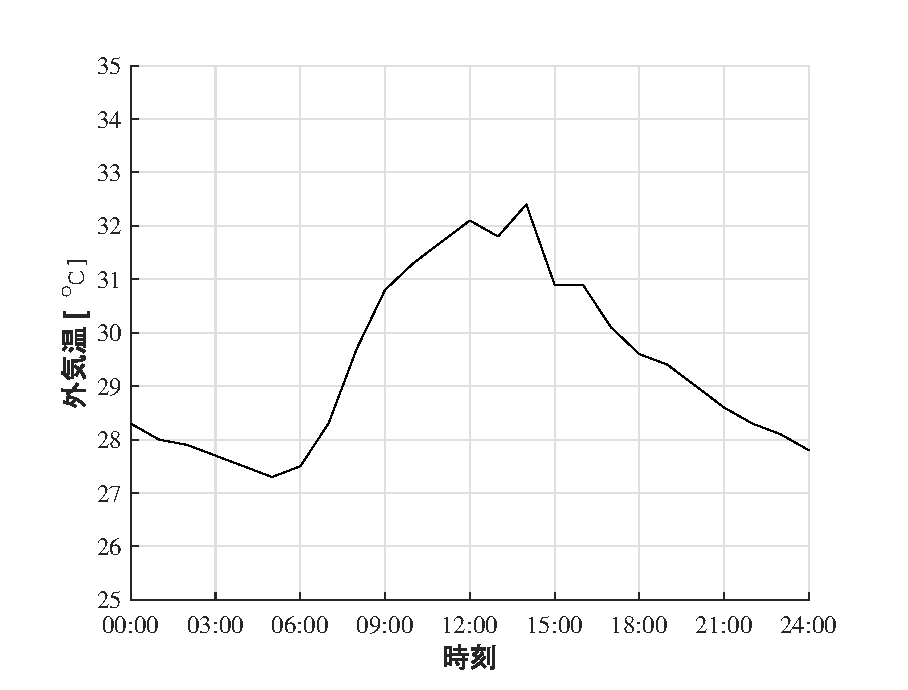
\includegraphics[width=0.7\linewidth]{fig/sim_outside_temp.eps}
  \end{center}
  \caption{一日の外気温の時間推移}
  \label{fig::sim_outside_temp}
\end{figure}

\begin{figure}[t]
  \begin{center}
    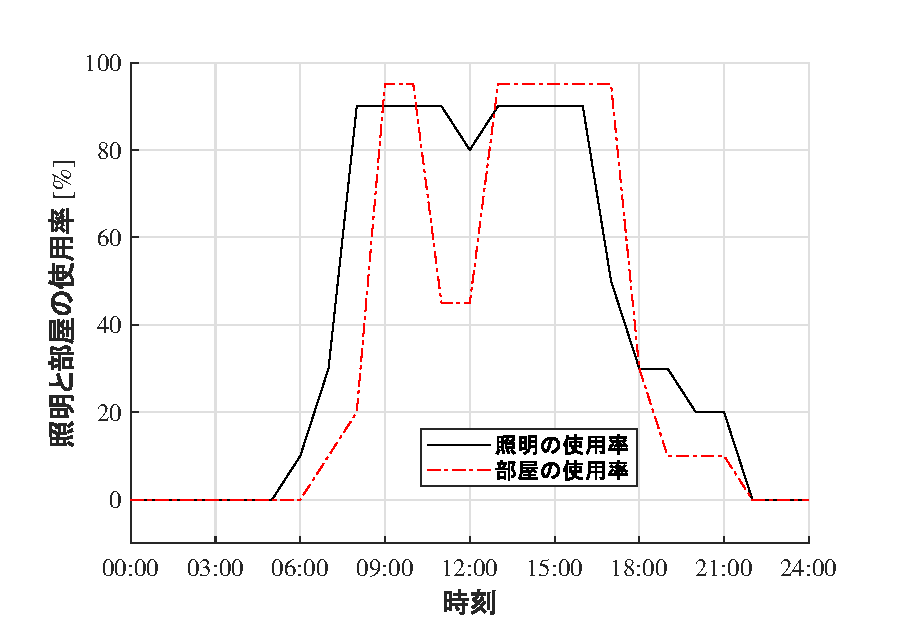
\includegraphics[width=0.7\linewidth]{fig/sim_occupancy.eps}
  \end{center}
  \caption{一日の照明と部屋の使用率の時間推移}
  \label{fig::sim_occupancy}
\end{figure}

\subsubsection{最適化部の設定}
OMOPSOで用いるパラメータを\tabref{tab::sim_param_omopso}に示す.本章では,EnergyPlusのシミュレーションを実行するプログラムとOMOPSOアルゴリズムをプログラミング言語Javaで実装した.計算機環境には,Windows 7 (64ビット),Intel Core i7-4790 (3.6GHz)およびRAM 8GBを用いた.

\begin{table}[ht]
  {\small
    \begin{center}
      \caption{OMOPSOのパラメータ}
      \label{tab::sim_param_omopso}
      \begin{tabular}{c|cccc}
        \hline
        パラメータ                             & 方法 / 値              \\
        \hline \hline
        ベース粒子群サイズ $N^{\mathcal{P}}$   & 50                     \\
        リーダー粒子群サイズ $N^{\mathcal{L}}$ & 100                    \\
        アーカイブ粒子群サイズ                 & 制限なし               \\
        総世代数 $g_{max}$                     & 500                    \\
        変数長 $n$                             & 20                     \\
        突然変異率 $p_m$                       & $1/n$                  \\
        重み $w$                               & [$0.1, 0.5$)の一様乱数 \\
        重み $c_1, c_2$                        & [$1.5, 2.0$)の一様乱数 \\
        非一様突然変異の係数 $b$               & 5 \cite{Esquivel03}    \\
        $\epsilon$-dominanceの係数$\epsilon$   & 0.0075                 \\
        \hline
      \end{tabular}
    \end{center}
  }
\end{table}


\section{実験結果}
\subsection{得られた空調設定スケジュール集合の目的関数値}
提案する空調最適化システムによって得られた設定温度スケジュール群の目的関数空間における分布を\figref{fig::sim_result_pareto}に示す.一つひとつの点が,一日の設定温度スケジュールであり,横軸を第1目的関数値の室内快適性,縦軸を第2目的関数値のエネルギー消費量とする空間にプロットされている.両方の目的関数値は,小さいほど良い結果と判断する.黒い点群は,提案する空調最適化システムによって一括獲得された最終世代のアーカイブ非劣粒子(設定温度スケジュール)群$\mathcal{E}$であり,粒子数は120だった.赤い×の点群は,従来システムとして,提案システムと同様に,エネルギーシミュレータに対して時間によらず設定温度が一定であるスケジュールを入力した場合の,快適度およびエネルギー消費量の算出結果である.

\figref{fig::sim_result_pareto}の結果から,提案法が,室内快適性およびエネルギー消費量のトレードオフを考慮した設定温度スケジュール集合を獲得できることがわかる.次に,動的に設定温度を変更する提案システムと設定温度を一定にする従来システムのスケジュールを比較する.一定の設定温度25.5[$^o$C]を用いる従来システムを除いて,提案システムは,室内快適性とエネルギー消費量の両方において,従来システムをパレート支配するスケジュールを獲得できることがわかる.

提案システムで得られたスケジュールBと温度設定を一定にする従来システムによるスケジュールDを比較する.提案システムによるスケジュールBは,従来システムによるスケジュールDと室内快適性は同程度だが,エネルギー消費量を約1.6\%削減できている.さらに,提案システムは,従来システムでは達成できない良好な室内快適性とエネルギー消費量のスケジュールを多数獲得できることがわかる.これは,双方の目的を両立するためには,設定温度を動的に変化させることが効果的であること,提案システムが適切な設定温度スケジュールを獲得できることを示している.
一方,一定温度25.5[$^o$C]を用いる従来システムによるスケジュールEは,提案システムによって得られたスケジュール集合ではパレート支配できない.しかし,一定温度25.5[$^o$C]を用いるスケジュールEは,室内快適性に関する制約条件\Eqref{eq::math_constraint_pmv}を満たさないことが確認された.すなわち,提案システムにおいて,スケジュールEは実行不可能解になる.そのため,提案システムは,従来システムによるスケジュールEをパレート支配するスケジュールを獲得できなかったと考えられる.

提案システムが獲得したスケジュールの効果をエネルギー消費量と快適性の2つの観点から試算する.従来法のスケジュールDを,同程度の快適性を示す提案法のスケジュールで置き換えると,エネルギー消費量を1日あたり$2.63×10^8$[J]削減できる.エネルギーが全て電力で賄われており,同様のエネルギー消費量削減を1年間継続できたとすると,1年間の電力消費量を約6,560[kWh],CO2排出量を3,850[kg]削減でき,オフィスビルの管理者に課せられたエネルギー消費量およびCO$_2$排出量の削減に貢献できる.また,同時に電気料金は1年間で約115,000円削減され,ビルオーナーの求める経済性にも寄与する.このシステムを全国のオフィスビルに適用でき,面積あたりの削減効果が同様だったとすると,全国のオフィスビルの総面積は約13,000[万$m^2$]である\cite{Fudoken19}ことから,全国で年間約12.7億円相当の電気料金削減と約42,400[t]のCO2排出量削減が可能である.一方で,従来のスケジュールDを同程度のエネルギー消費量の提案法のスケジュールで置き換えると,快適度が0.07向上する.これは,快適度が不快側であった場合に比べて0.875\%のオフィスワーカーの生産性改善につながる\cite{Iwahashi14, WGBC14}.今回の対象ビルのオフィスワーカーの人数は827人であり,それぞれに平均年収と同額の人件費(441万円)\cite{NTA19}がかかっている場合,約2,130万円の生産性改善効果が見込める.このシステムを全国のオフィスビルに適用できると,全国で約1,000万人存在するオフィスワーカー\cite{Fudoken19, Xymax19}全体で約2,720億円の生産性改善効果があると考えられる.

これらの結果から,提案システムは,従来システムによる一定温度設定より,室内快適性とエネルギー消費量が良好な設定温度スケジュールを獲得できることが明らかになった.

\begin{figure}[htbp]
  \begin{center}
    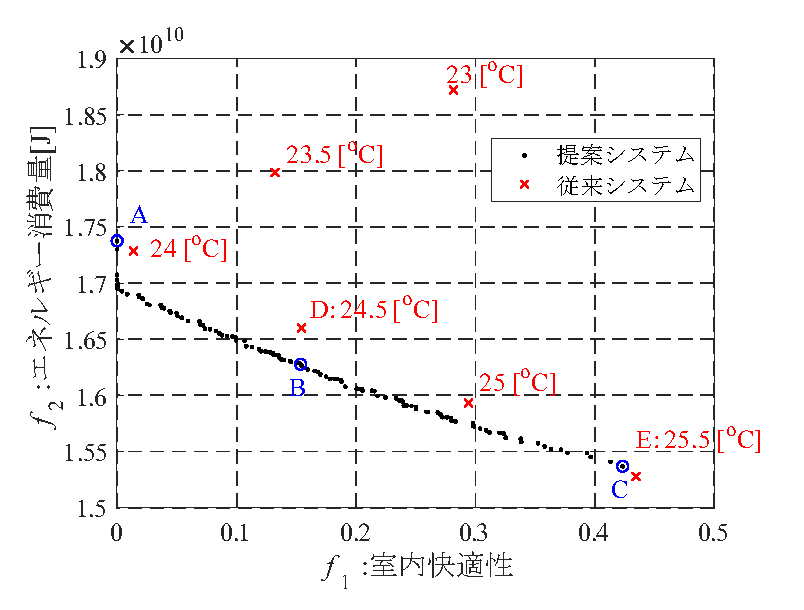
\includegraphics[width=0.7\linewidth]{fig/sim_result_pareto.eps}
  \end{center}
  \caption{シミュレーション最適化の結果}
  \label{fig::sim_result_pareto}
\end{figure}

\begin{figure*}[htbp]
  \begin{center}
    \begin{minipage}{0.5\textwidth}
      \begin{center}
        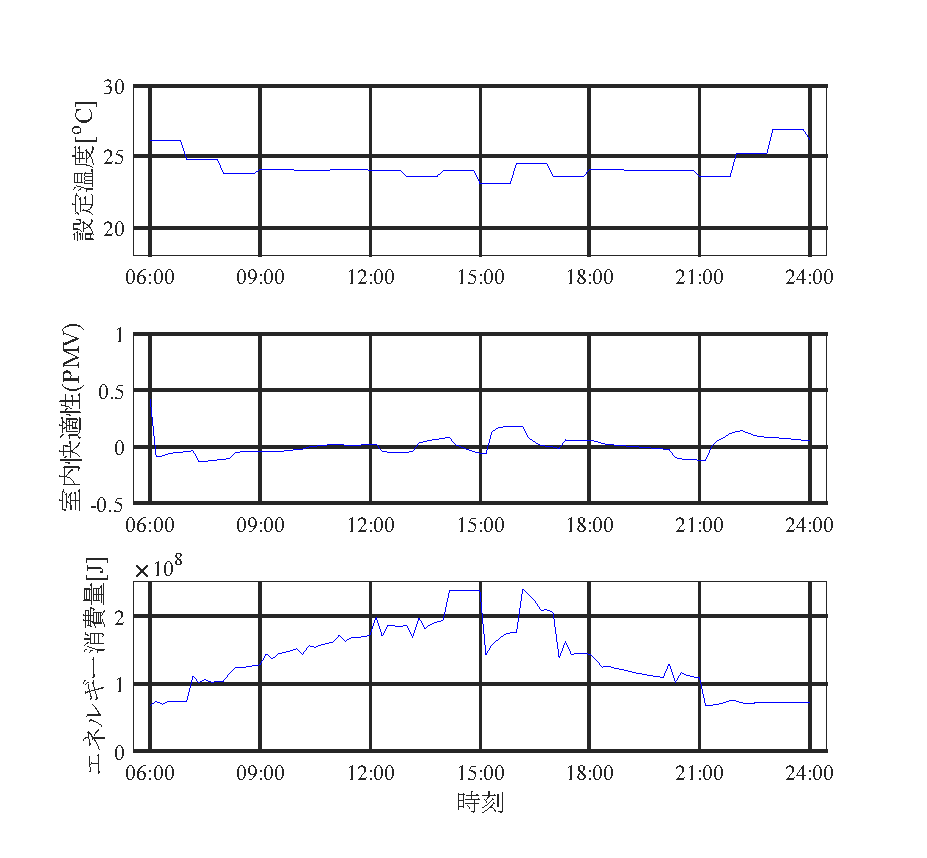
\includegraphics[width=1.0\textwidth,keepaspectratio=true]{fig/sim_result_schedule_a.eps}\\\vspace{-2mm}{スケジュール A (室内快適性が最も良い解)}
      \end{center}
    \end{minipage}
    \begin{minipage}{0.5\textwidth}
      \begin{center}
        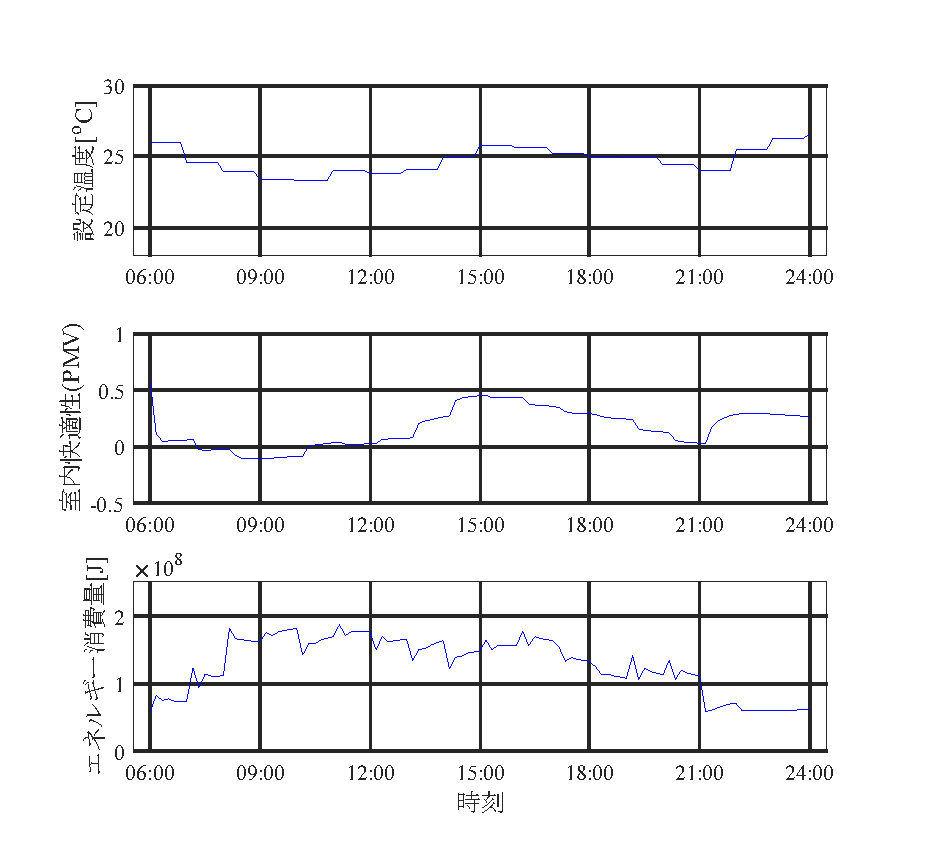
\includegraphics[width=1.0\textwidth,keepaspectratio=true]{fig/sim_result_schedule_b.eps}\\\vspace{-2mm}{スケジュール B (中間の解)}
      \end{center}
    \end{minipage}
    \begin{minipage}{0.5\textwidth}
      \begin{center}
        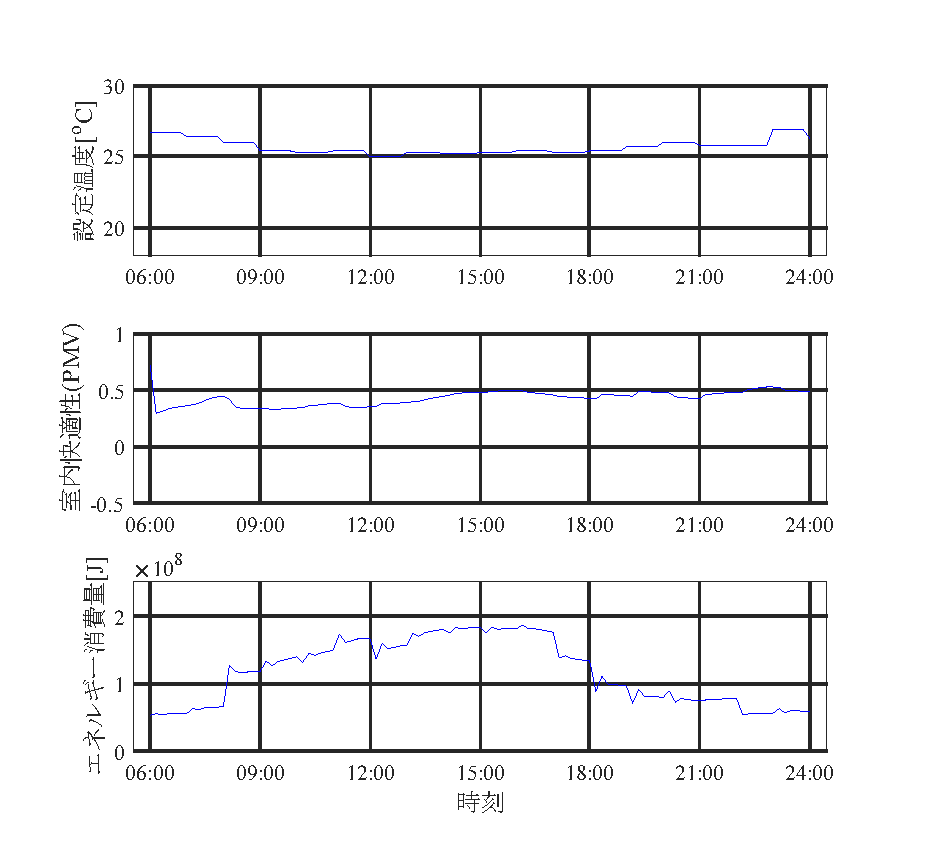
\includegraphics[width=1.0\textwidth,keepaspectratio=true]{fig/sim_result_schedule_c.eps}\\\vspace{-2mm}{スケジュール C (室内快適性が最も悪い解) }
      \end{center}
    \end{minipage}
  \end{center}
  \vspace{-2mm}
  \caption{提案システムで得られた設定温度スケジュールによる結果}
  \label{fig::sim_result_schedule}
\end{figure*}

\begin{figure*}[htbp]
  \begin{center}
    \begin{minipage}{0.5\textwidth}
      \begin{center}
        \includegraphics[width=1.0\textwidth,keepaspectratio=true]{fig/sim_result_schedule_d.eps}\\{スケジュール D (設定温度24.5[$^o$C])}
      \end{center}
    \end{minipage}
    \hspace{2cm}
    \begin{minipage}{0.5\textwidth}
      \begin{center}
        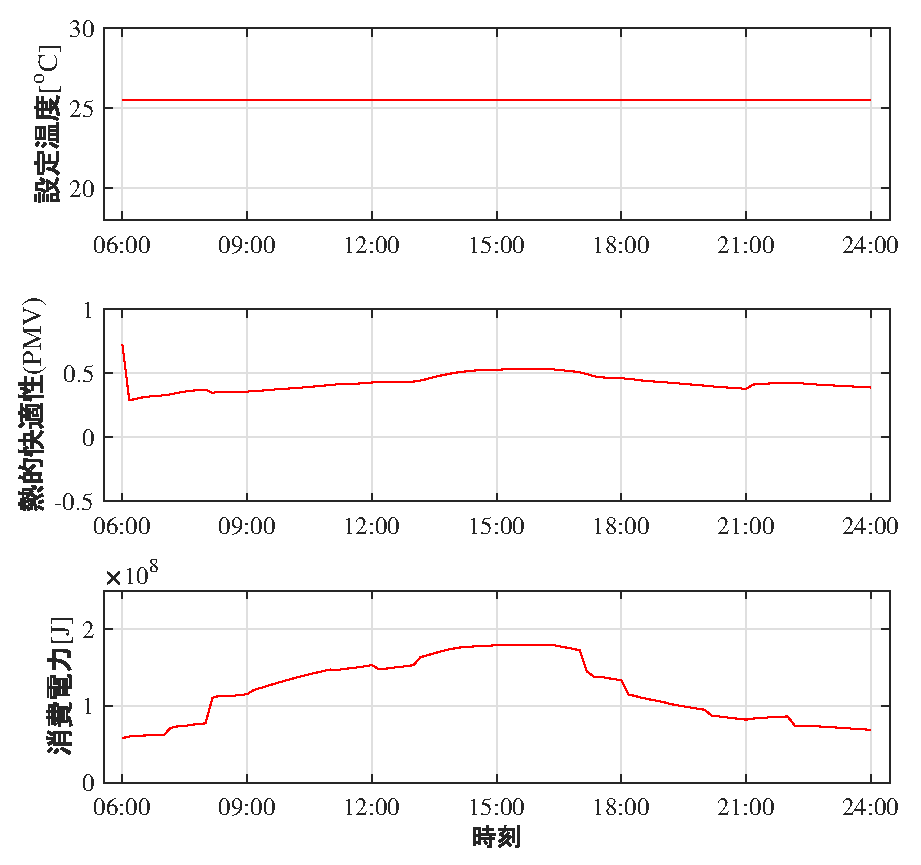
\includegraphics[width=1.0\textwidth,keepaspectratio=true]{fig/sim_result_schedule_e.eps}\\{スケジュール E (設定温度25.5[$^o$C])}
      \end{center}
    \end{minipage}
  \end{center}
  \vspace{2mm}
  \caption{従来システムで得られた設定温度スケジュールによる結果}
  \label{fig::sim_result_schedule_const}
\end{figure*}

\subsection{得られた設定温度スケジュールの時系列データ}\label{subsec::sim_schedule_timeseries}
\subsubsection{従来システムによる設定温度一定のスケジュールとの比較}
得られた設定温度スケジュールの時系列データについて議論する.\figref{fig::sim_result_pareto}において青い円で示した提案システムによる設定温度スケジュールA,B,Cについて,設定温度,室内快適性(PMV値),エネルギー消費量の時系列データを\figref{fig::sim_result_schedule}に示す.Aは最も快適だがエネルギー消費量が高いスケジュール,Cは最もエネルギー消費量が低いが快適性が低いスケジュール,Bは中間のバランスされたスケジュールとして\figref{fig::sim_result_pareto}から取り出した.また,従来システムによるDとEの時系列データを\figref{fig::sim_result_schedule_const}に示す.\figref{fig::sim_result_schedule}と\figref{fig::sim_result_schedule_const}において,室内快適性としてプロットした値は,範囲[-3, +3]のPMV値であり,\Eqref{eq::math_objective1}において第1目的関数の定式化に利用したPMV値の絶対値ではないことに注意されたい.そのため,ここでは,PMV値がゼロの場合に最も快適であり,マイナス値は寒さによって快適性が低下し,プラス値は暑さによって快適性が低下すると判断する.

まず,設定温度の時系列データについて,\figref{fig::sim_result_schedule_const}の従来システムが設定温度を一定にするのに対して,\figref{fig::sim_result_schedule}の提案システムは時刻の変化に伴って設定温度を動的に変更することがわかる.\figref{fig::sim_result_schedule_const}における従来システムの結果から,温度設定を一定にすると,15:00まで暑さによってPMV値が上昇し,同様にエネルギー消費量も上昇することがわかる.日中の外気温の上昇が,空調の熱源に生成する熱量の増加と効率の悪化を招き,エネルギー消費量が増加する.次に,室内快適性に関する第1目的関数値が同程度の提案システムによるスケジュールBと従来システムによるスケジュールDを比較すると,提案システムによるスケジュールBは,午前中に空調の設定温度を低下させ,15:00には設定温度を上昇させることで空調システムの負荷を低減させる.提案システムでは,設定温度の変更に伴い,熱源の生成する熱量が変化するため,空調システムのエネルギー消費量が変化する.これにより,午前中のエネルギー消費量は,設定温度を一定にする従来システムより高くなるが,15:00付近のエネルギー消費量は抑制される.その結果,\figref{fig::sim_result_pareto}に示したように,提案システムによるスケジュールBは,従来システムのスケジュールDより総エネルギー消費量を抑制できる.設定温度が一定の従来システムによるエネルギー消費量の変化は緩やかだが,設定温度を変更する提案システムの場合,設定温度を変更するタイミングでエネルギー消費量が急激に変化する傾向が見て取れる.しかし,提案システムは,このエネルギー消費量の急峻な増減が発生しても,一日の総エネルギー消費量としては低くなるスケジュールを生成している.また,従来システムによるスケジュールEについては,14:00~17:00の間に快適度が0.5を超過しており,制約条件\Eqref{eq::math_constraint_pmv}を満たしていないことが確認できる.

\figref{fig::sim_result_schedule}の室内快適性が低いスケジュールCは,PMV値が終日0.5に近い値で推移することがわかる.一方,\figref{fig::sim_result_schedule}の室内快適性が高いスケジュールAは,PMV値がゼロに近い値を維持することがわかる.スケジュールAは,14:00~16:00の外気温が高く,空調システムの効率が悪化してエネルギー消費量が上昇しやすい時間帯に温度設定を上げることにより,PMV値を上昇させてエネルギー消費量の増加を抑制することがわかる.

\begin{figure*}[htbp]
  \begin{center}
    \begin{minipage}{0.5\textwidth}
      \begin{center}
        \includegraphics[width=1.0\textwidth,keepaspectratio=true]{fig/sim_result_schedule_a_settemp_diff.eps}\\{(a) スケジュールAとその隣接解}
      \end{center}
    \end{minipage}
    \begin{minipage}{0.5\textwidth}
      \begin{center}
        \includegraphics[width=1.0\textwidth,keepaspectratio=true]{fig/sim_result_schedule_b_settemp_diff.eps}\\{(b) スケジュールBとその隣接解}
      \end{center}
    \end{minipage}
    \begin{minipage}{0.5\textwidth}
      \begin{center}
        \includegraphics[width=1.0\textwidth,keepaspectratio=true]{fig/sim_result_schedule_c_settemp_diff.eps}\\{(c) スケジュールCとその隣接解}
      \end{center}
    \end{minipage}
  \end{center}
  \vspace{-2mm}
  \caption{提案システムで得られた設定温度スケジュールの隣接解との差}
  \label{fig::sim_result_schedule_settemp_diff}
\end{figure*}

\subsubsection{獲得した設定温度スケジュールの特徴}
次に,提案システムで得られた設定温度スケジュールにどのようなパターンが存在するか分析する.\figref{fig::sim_result_schedule_settemp_diff}に,提案システムで得られた設定温度スケジュールA, B, Cと,その両隣に隣接したスケジュールA', A'', B', B'', C', C''のスケジュールを示す.\figref{fig::sim_result_schedule_settemp_diff}を見ると,設定温度スケジュールB,Cの近くには,概ねそれらのスケジュールに近い設計変数を持つ解しか存在しないのに対して,設定温度スケジュールAの近くにはAとは大きく異なる設計変数を持つ多様なスケジュールが存在する.
\red{定量的にこのスケジュールの多様性を評価するため,以下の\Eqref{eq::sim_mulltimodal_index}で定める$I_d$という評価尺度を導入する.
  \begin{eqnarray}
    I_d &= \frac{1}{100} \sum^{10}_{i=1} \sum^{10}_{j=1}(D_{i, j} - \bar{D})^{2}
    \label{eq::sim_mulltimodal_index}
  \end{eqnarray}
  ここで,$D_{i, j}$は,次の\Eqref{eq::sim_setpoint_distance}で定義される.この式は,ある設定温度スケジュール集合における$i$番目の設定温度$t_{set}^{i}(t)$と$j$番目の設定温度$t_{set}^{j}(t)$の各時刻の差の絶対値の総和であり,設計変数間の距離を表す.$\bar{D}$は,設定温度スケジュール集合の各設計変数間の距離の平均値である.
  \begin{eqnarray}
    D_{i, j} &= \sum^{n}_{t=1} |t_{set}^{i}(t) - t_{set}^{j}(t)|
    \label{eq::sim_setpoint_distance}
  \end{eqnarray}
  $I_d$はある設定温度スケジュール10個の設計変数間の距離の分散であり,この値が大きいほど設計変数が多様であることを示す.この多様性評価尺度$I_d$を提案システムで得られた設定温度スケジュールA, B, C付近の設計変数10個ずつを抽出してそれぞれに対して計算し正規化すると,設定温度スケジュールA付近では$I_d=1.0$であるのに対し,設定温度スケジュールB付近では$I_d=0.28$,設定温度スケジュールC付近では$I_d=0.1$となった.この結果から,定量的にも,設定温度スケジュールAの近くにはAとは異なる多様な設定温度スケジュールが存在し,設定温度スケジュールB,Cの近くにはそれらのスケジュールに近いスケジュールしか存在しないことがわかる.
}

この結果は,本章で扱う空調設定温度スケジュール最適化問題が,スケジュールA付近では離れた設計変数でも目的関数が良い点が存在する多峰性を持った関数であることを示唆している.これは,スケジュールCなどの制約条件に近いスケジュールの場合,設定温度を多少変更しただけで制約違反となってしまうことから,制約を満たしつつ目的関数を良くする設定温度スケジュールのパターンが制限されて一意に決まってくるのに対し,スケジュールA付近では多少の設定温度変更をしても制約違反とはなりにくく,様々な設定温度スケジュールのパターンによって目的関数を良くすることが可能であることが理由と考えられる.

異なる設計変数(スケジュール)が,同一もしくは類似した目的関数値を示す最適化問題をマルチモダル(Multimodal, 多峰性)最適化問題\cite{Tanabe20}という.目的関数空間におけるスケジュールAの周辺には,マルチモダル最適化の問題クラスに相当する傾向がみられることがわかった.提案システムは,このような多峰性を持つ問題であっても局所解に陥らず複数のパターンの中から他のパターンを優越する解を探索できているため,\figref{fig::sim_result_schedule_settemp_diff}(a)のように多様なパターンを解集合に含んでいるものと考える.
\red{これに対し,スケジュールB, Cの周辺は,似通った設計変数(スケジュール)が類似した目的関数値を示す.このような最適化問題をユニモダル(Unimodal, 単峰性)最適化問題と呼ぶ.空調設定温度スケジュール最適化問題は,目的関数空間のエリアによってマルチモダルおよびユニモダル最適化問題のそれぞれ異なる特性をもつ問題となっている.提案システムは,スケジュールAの近傍のマルチモダルな傾向の範囲だけではなく,スケジュールB, Cの近傍のユニモダルな傾向を持つ範囲であっても良好な解を探索できている.}

\red{
ここで,他のビルでも同様な傾向にあるか確認するため,以下の\figref{fig::sim_office_building_small}に示す小規模オフィスビルのシミュレーションモデルを用意し,提案システムによって空調設定温度スケジュールの多目的最適化を行った.この小規模オフィスビルモデルの対象は,地上1階建ての5つの部屋を持つ建物で,延床面積が464[$m^2$]である.床面積とフロアレイアウト以外のモデル設定は,\secref{sec::sim_model}で述べたオフィスビルモデルと同様である.また,最適化アルゴリズムおよび最適化部の設定は\secref{sec::sim_setting}と同様とした.
}
\begin{figure}[htbp]
  \begin{center}
    \vspace{-4mm}
    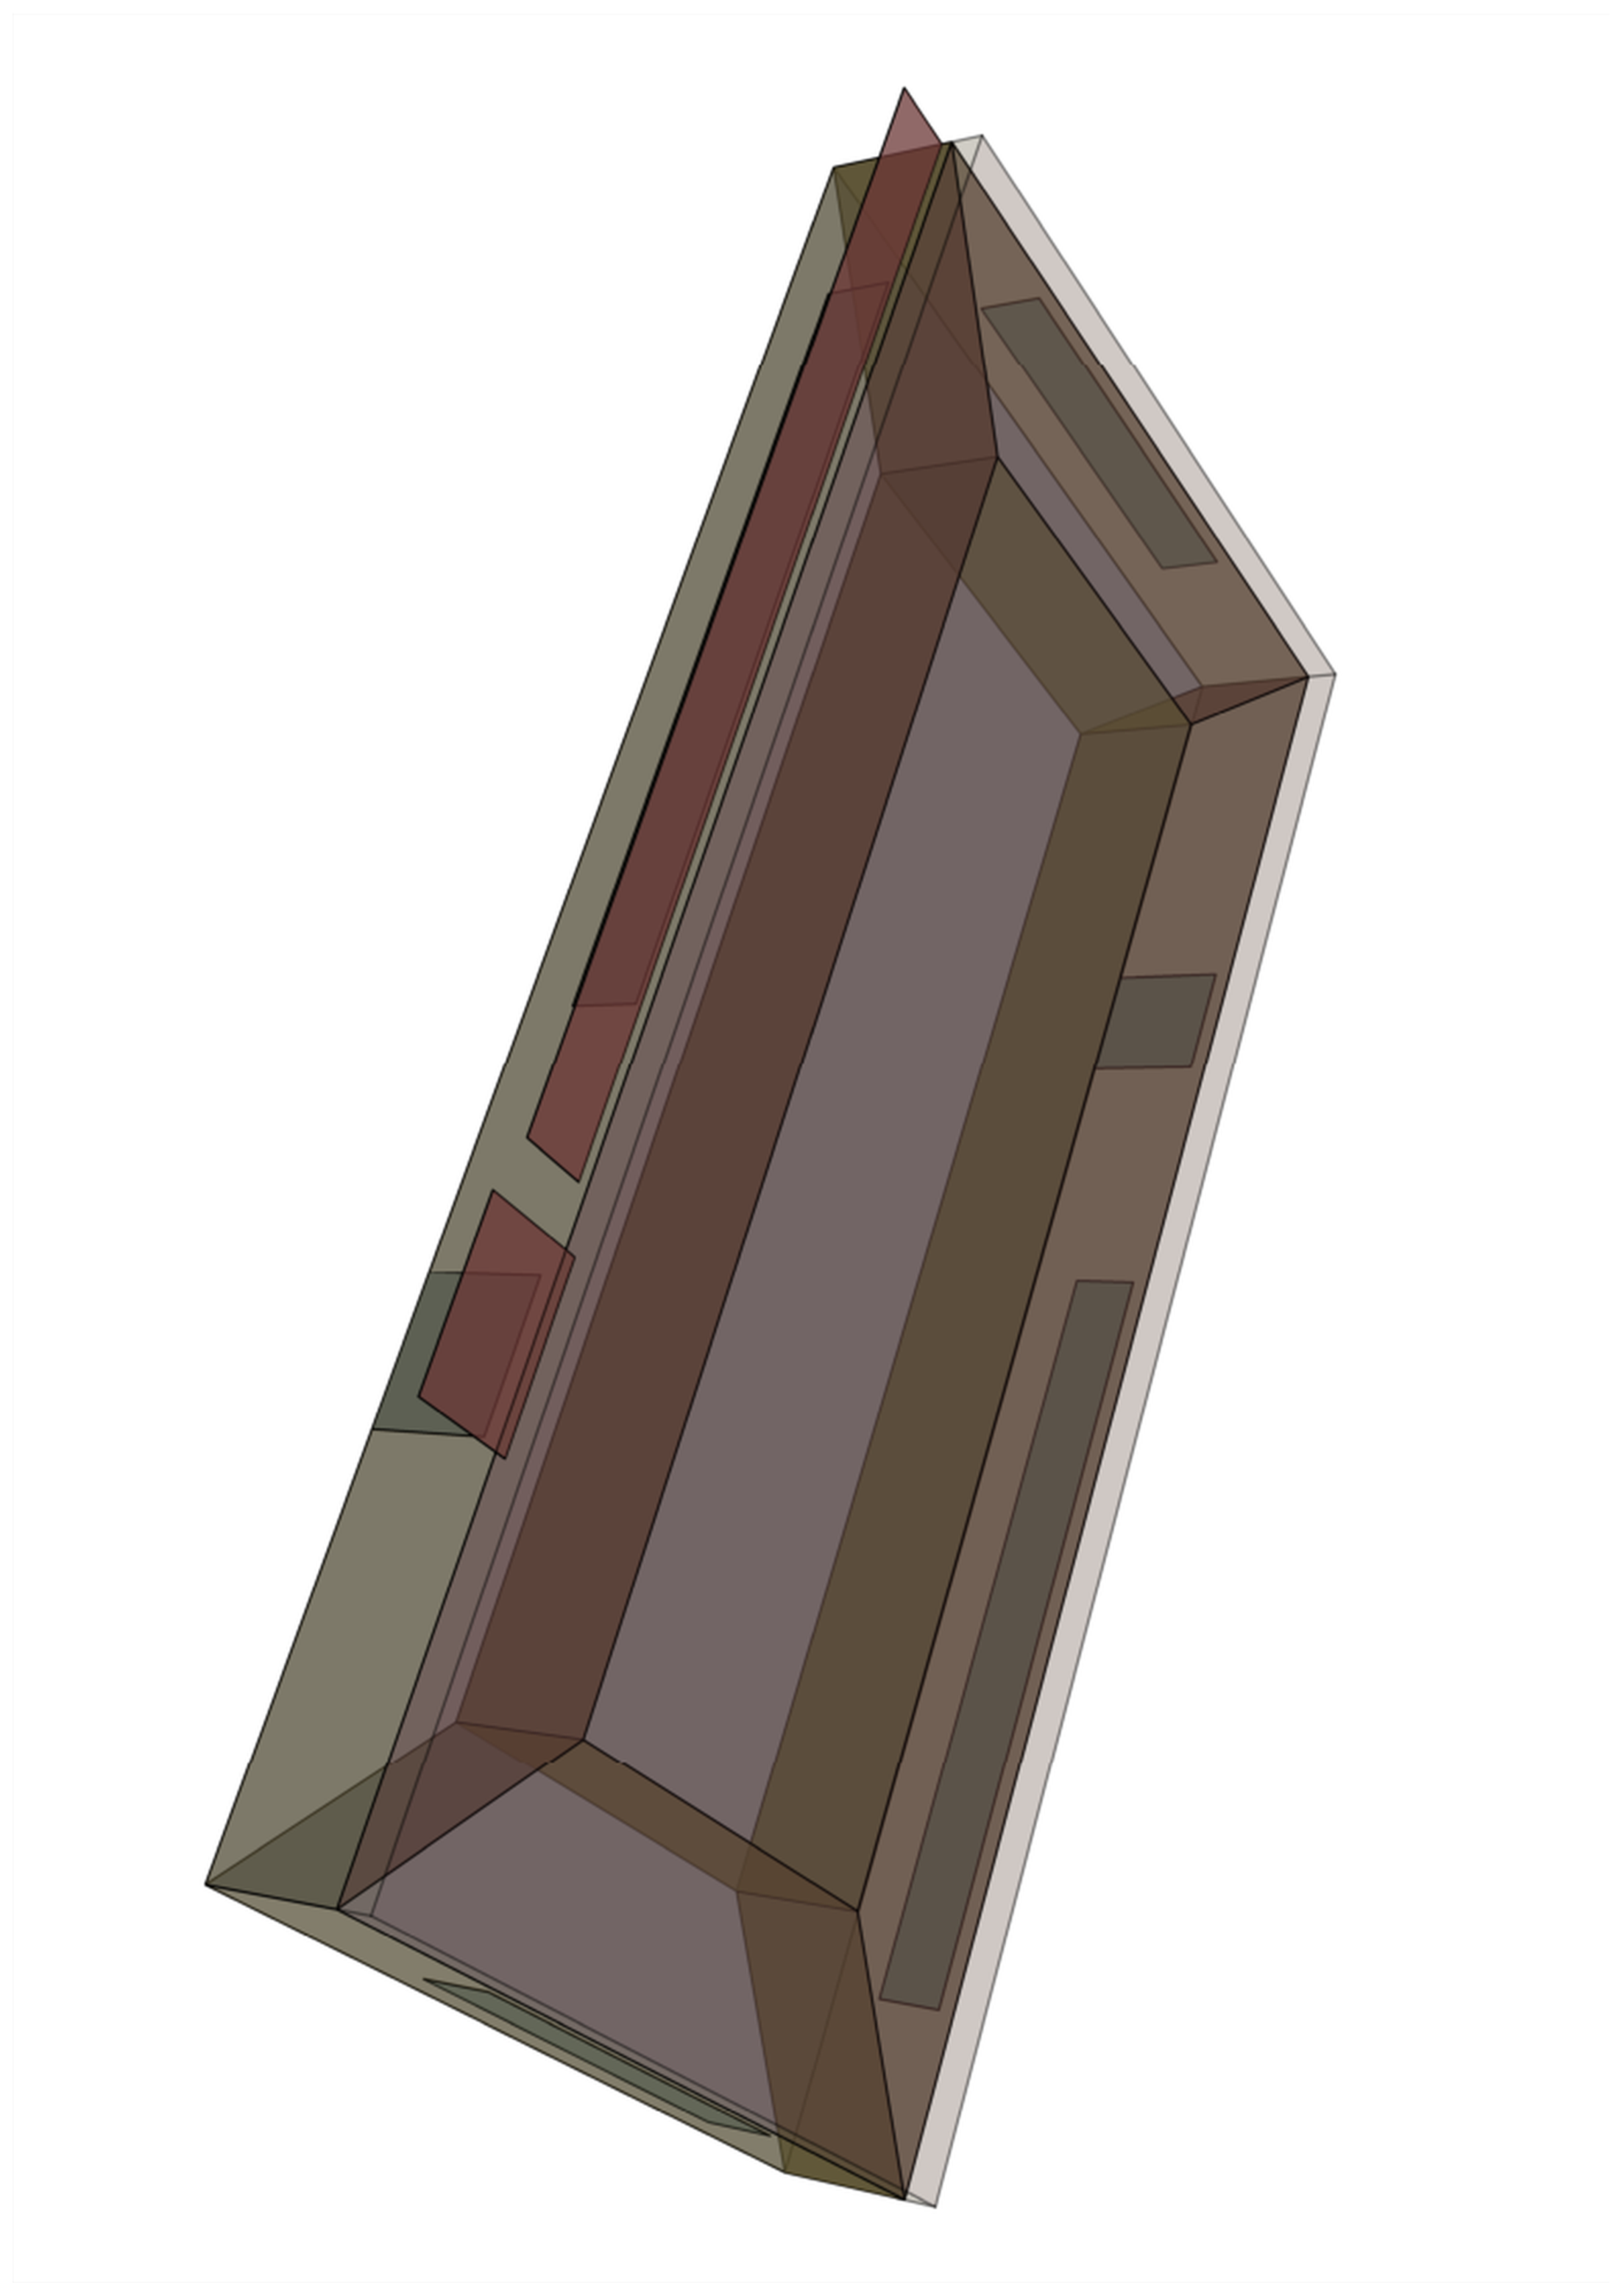
\includegraphics[width=0.6\linewidth, angle=90]{fig/sim_office_building_small.eps}
  \end{center}
  \vspace{-15mm}
  \caption{小規模オフィスビルモデルの外観}
  \label{fig::sim_office_building_small}
\end{figure}
\red{
  小規模オフィスビルシミュレーションモデルに対する多目的最適化を行い獲得した空調設定スケジュールを\figref{fig::sim_result_pareto_small}に示す.また,\figref{fig::sim_result_pareto_small}において,\figref{fig::sim_result_pareto}と同様に快適,不快,中間の室内快適性を持つスケジュールF, G, Hを抽出し青の円で示した.スケジュールF,G,Hそれぞれの付近の設計変数10個ずつに対して,スケジュールの多様性評価尺度$I_d$を計算し正規化すると,スケジュールF付近では$I_d=1.0$,スケジュールG付近では$I_d=0.57$,スケジュールH付近では$I_d=0.38$となった.この結果から,小規模オフィスビルでも中規模オフィスビルと同様に,目的関数空間に獲得されたスケジュールが多様であるエリアとそうではないエリアがある,マルチモダルおよびユニモダル最適化問題それぞれの異なる特性をもつ問題となっていることが確認できる.一方で,小規模オフィスビルの多目的最適化結果では,室内快適性に関する目的関数値が$0.24 \leq f_1 \leq 0.5$の解は得られていない.この理由は,ビル規模により快適性に関する制約条件\Eqref{eq::math_constraint_pmv}を満たすことの容易さに違いがあるためであると考える.規模の大きいビルでは,部屋の空間が広く,躯体も耐震性を配慮し強度の高いコンクリートが多分に使用されており,空調対象室の熱容量が大きい.そのため,設定温度変更に対して,室内温度・壁面温度が変化しにくく,快適性の変化は遅くなる.冷房条件では,空調負荷の高い日中帯は特に快適性の変化が遅くなるため,設計変数である設定温度を大きく変更しても制約の境界値を超過しにくい.結果として得られる温度スケジュールは多様性が高いものが多い傾向になる.一方で,小規模なビルでは空調対象室の熱容量が小さく,設定温度変更に対して快適性が急峻に変化する.空調機の特性によってはオーバーシュートやハンチングを起こすこともあるため,制約違反しやすい.このように制約を容易には満足できないため,制約の境界に近い$0.24 \leq f_1 \leq 0.5$の範囲では解を獲得できておらず,結果として得られる制約を満たした温度スケジュールは似通ったものが多い傾向になるものと考える.この小規模オフィスビル最適化問題は,最適化手法から見ると,制約を満たすことが難しいため探索により良好な解を獲得することが難しい問題であるといえる.しかし,このような難しさのある小規模オフィスビルの空調設定スケジュール最適化問題に対しても,提案システムは快適性とエネルギー消費量のトレードオフを近似する良好なパレート解候補を獲得できている.他の規模・フロアレイアウトや断熱材・空調システムなどの設定を持つオフィスビルにおいても,上述の中規模オフィスビル・小規模オフィスビルモデルと同様の問題クラスを持つとすれば,それらのオフィスビルにも提案システムが有効である可能性がある.
}

\begin{figure}[htbp]
  \begin{center}
    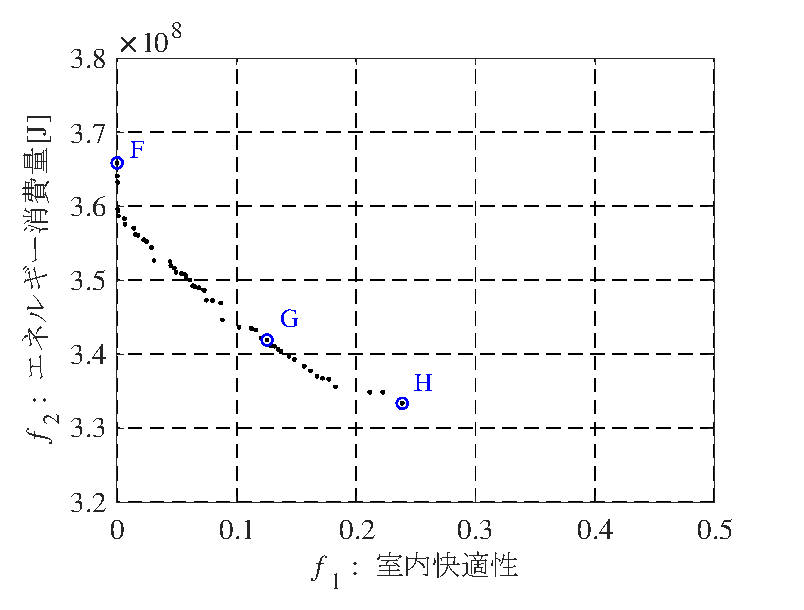
\includegraphics[width=0.7\linewidth]{fig/sim_result_pareto_small.eps}
  \end{center}
  \caption{小規模オフィスビルモデルのシミュレーション最適化の結果}
  \label{fig::sim_result_pareto_small}
\end{figure}

\subsection{計算時間}
本章の計算機実験の環境において,各粒子(スケジュール)を評価するEnergyPlusのシミュレーションには約40秒かかる.各評価シミュレーションを8並列で実行し,最適化の実行時間は37時間31分だった.このように,現在の計算機環境における提案システムでは,空調の設定温度スケジュールを得るために,約1.5日前に最適化を実行する必要がある.外気温予報などの入力データの精度は,予測時点が近いほど高まる.より精度が高い予報を含む入力データを利用するためには,より高速にシミュレーションを実行することが必要になる.このためには,シミュレーションの高速化やPCクラスタなどを導入した並列度の高い計算機環境を用いる手段などが考えられる.

\section{提案システム設計の妥当性検証}\label{sec::sim_valid}
提案システムの設計について,室内快適性に関する制約条件を設ける効果,$\epsilon$制約法による単一目的最適化との比較による多目的最適化する効果,異なる多目的進化計算法を用いたときの効果,OMOPSOによるアルゴリズム上の工夫の効果について議論する.

\subsection{制約条件を設ける効果}
\subsubsection{目的}
本論文の提案システムにおいて,室内快適性に関する制約条件\Eqref{eq::math_constraint_pmv}を設ける意義について検証する.一般的に,制約条件が,必ずしも満たす必要はないものの可能な限り満たしたいソフト制約の場合や,必ず満たさなければならないハード制約であっても実行可能解の獲得が困難な場合,最適化の過程で制約条件は考慮せず,獲得した解集合から制約条件を満たさない解を除去したり,制約条件に近い解を意思決定者に提示したりすることがある.この方法によって,最適化の過程で制約条件を考慮しなければ,より多様な解の探索が可能になるが,制約条件を考慮した最適化より実行可能解は得られにくくなる.本項では,制約条件を考慮する方法と考慮しない方法によって得られた解集合を比較することで,提案システムにおいて制約条件\Eqref{eq::math_constraint_pmv}を設ける意義と効果を明らかにする.

\begin{figure}[htbp]
  \begin{center}
    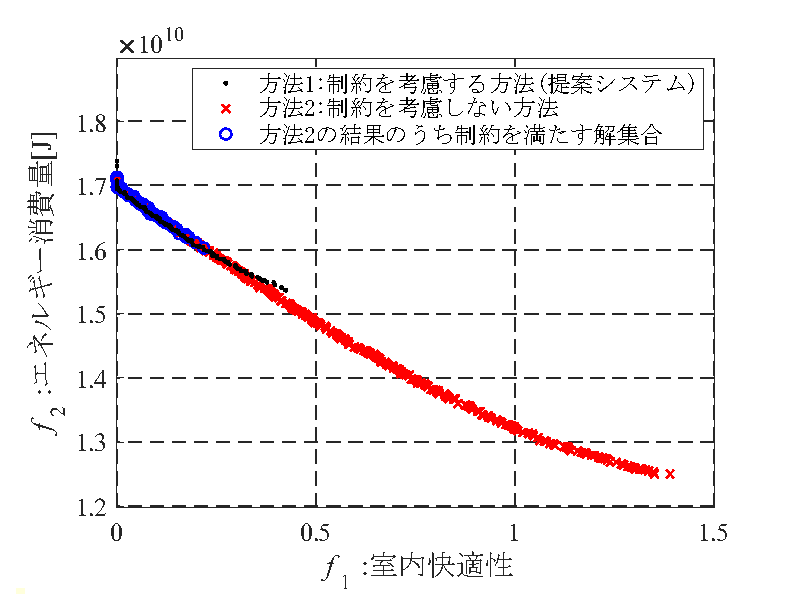
\includegraphics[width=0.7\linewidth]{fig/sim_result_pareto_cc.eps}
  \end{center}
  \caption{制約条件\Eqref{eq::math_constraint_pmv}の考慮の有無によって得られた解集合}
  \label{fig::sim_result_pareto_cc}
\end{figure}

\subsubsection{方法}
最適化の過程で,制約条件\Eqref{eq::math_constraint_pmv}を考慮する方法1,考慮しない方法2を比較する.方法1は,提案システムである.方法1と2は,ともに\tabref{tab::sim_param_omopso}に示すパラメータを用いる.


\subsubsection{結果}
得られた解集合の目的関数空間における分布を\figref{fig::sim_result_pareto_cc}に示す.この結果から,制約条件\Eqref{eq::math_constraint_pmv}を考慮しない方法2は,$f_1$値が高く快適性は悪いもののエネルギー消費量を抑制できるスケジュールを獲得できることがわかる.方法2が獲得した解集合の中で,制約条件\Eqref{eq::math_constraint_pmv}を満足する解集合に青い円で印をつけた.青い円の解集合は,最適化の過程で制約条件\Eqref{eq::math_constraint_pmv}を考慮する方法1による解集合と比較すると,エネルギー消費量が低くならないことがわかる.これは,第1目的関数における一日の室内快適性の平均値の最小化を試みても,方法2では,制約条件\Eqref{eq::math_constraint_pmv}における計測時刻ごとの室内快適性を満たしつつ第2目的関数であるエネルギー消費量が低いスケジュールを獲得することには困難があるといえる.提案システムである方法1は,制約条件\Eqref{eq::math_constraint_pmv}を設けることで,室内快適性の良好な解の獲得を促進し,その条件下でエネルギー消費量が低いスケジュールを獲得できたといえる.


\subsection{多目的最適化と$\epsilon$制約法による単一目的最適化}
\subsubsection{目的}
本論文の提案システムにおいて,室内快適性とエネルギー消費量を多目的に最適化する意義について検証する.多目的最適化する利点のひとつは,室内快適性とエネルギー消費量のトレードオフ関係をビル管理者に提示し,長期的なエネルギー消費計画と合わせて実行する設定温度スケジュールを意思決定させるためである.しかし,利用するスケジュールは,獲得した多様なスケジュール集合のうちの一つだけであり,利用しないスケジュールに探索計算コストをかけることになる.最適化に関する選好情報を利用し,単一目的最適化によって一つの解を求めることで,トレードオフになる多様なスケジュール集合は獲得しない手段も考えられる.本項では,本論文の空調最適化問題を単一目的最適化する方法と多目的最適化する方法を比較する.

\subsubsection{方法}
多目的最適化問題を単一目的最適化問題にして解く方法として,$\epsilon$制約法\cite{Haimes71}を取り上げる.$\epsilon$制約法は,複数の目的関数のうちいくつかに許容値を設けて制約条件とし,残りの目的関数を最適化する.本項では,次式による$\epsilon$制約法によって,多目的最適化問題である空調スケジュール最適化問題を単一目的最適化問題に変換する.
\begin{eqnarray}
  \begin{cases}
    \mbox{Minimize} \quad f_2(\vec{x})                  & \\
    \mbox{Subject\ to} \quad f_1(\vec{x}) \leq \epsilon & \\
  \end{cases}
\end{eqnarray}
すなわち,室内快適性に関する目的関数$f_1$に最大値$\epsilon$を与えることで制約条件にし,エネルギー消費量に関する目的関数$f_2$を最小化する単一目的最適化問題にする.本項では,$\epsilon = \{0.01, 0.1, 0.2, 0.3, 0.4\}$とし,5つの選好解を求めることにした.

単一目的最適化手法として,PSOと差分進化(Differential Evolution, DE) \cite{Price06}を用いた.
提案システムにおける多目的最適化のためのOMOPSOと比較するため,単一目的最適化のためのPSOには,ひとつの目的関数を扱うOMOPSOを用いる.単一目的最適化のため,リーダー粒子群$\mathcal{L}$およびアーカイブ粒子群$\mathcal{E}$のサイズを1にし,各世代で最良の目的関数値を持つ粒子をリーダーにすること以外は,提案システムにおける多目的最適化のためのOMOPSOと同じ設定を用いる.また,DEにおける解の生成法には,rand/1/binを用い,個体数50,総世代数500として,解の評価回数を等しくした.交叉率は$C_r=0.9$,スケーリング係数は$F=0.7$にした.単一目的最適化のPSOとDEの両方において,制約条件を伴う解の比較について,比較する2つの解が実行可能なら目的関数値$f_2$が良い方,片方が実行可能でもう片方が実行不能なら実行可能の方,2つの解が実行不可能なら$f_1$が$\epsilon$に近い方が良いと判断した.

ここで,本項で用いるPSOとDE,これらに利用するアルゴリズムのパラメータ,さらには単一目的化するための$\epsilon$制約法と制約条件の取り扱い方は,空調スケジュール最適化問題の単一目的最適化のために最良というわけではなく,単一目的最適化の手段の例として取り上げることに注意されたい.空調スケジュール最適化問題を含む実世界問題には,一つひとつの解の評価に時間を要するものがあり,最良の方法とパラメータを試行錯誤して見出すことは実質的に困難である.そのため,本項における単一目的最適化のためのPSOは,多目的最適化のためのOMOPSOと比較するために採用しており,DEも基礎的かつ一般的な方法とパラメータを採用している.

\begin{figure}[htbp]
  \begin{center}
    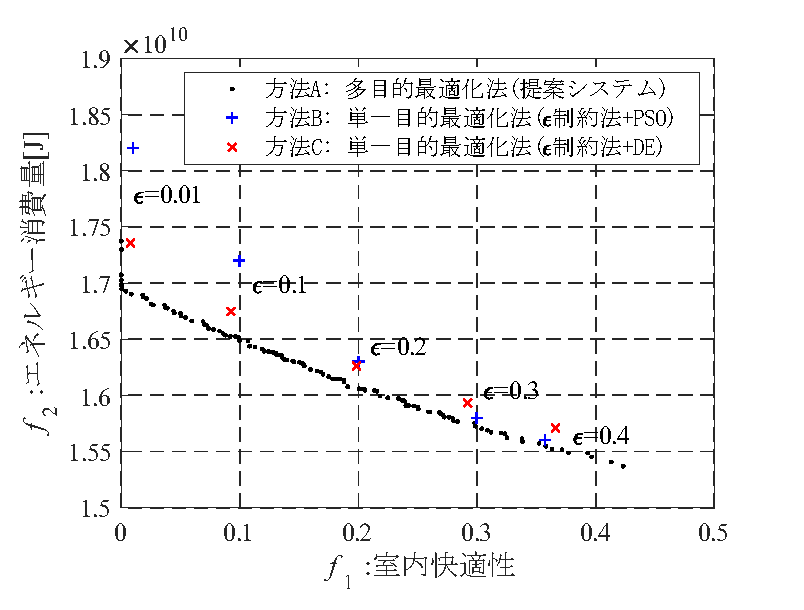
\includegraphics[width=0.7\linewidth]{fig/sim_result_pareto_multisingle.eps}
  \end{center}
  \caption{ 多目的最適化と$\epsilon$制約法に基づく単一目的最適化によって得られた解集合}
  \label{fig::sim_result_pareto_multisingle}
\end{figure}

\subsubsection{結果}
多目的最適化する提案システムを方法A,単一目的最適化する$\epsilon$制約法を組み込んだPSOを方法B,同じく$\epsilon$制約法を組み込んだDEを方法Cとし,得られた解集合を\figref{fig::sim_result_pareto_multisingle}に示す.方法Aは1回の実行結果,方法BとCは$\epsilon$が異なる5回の実行結果を示す.

まず,単一目的最適化する方法BとCを比較する.$\epsilon=0.4$を用いる場合,方法Bによる解は,方法Cによる解をパレート支配する.しかし,これら2つの解は,$f_1=0.4$近くまで到達できない.このように,$\epsilon$制約法において,$\epsilon$が大きい場合,$\epsilon$制約の境界近くに解を獲得しにくい傾向が見られた.$\epsilon=\{0.01,0.1\}$を用いる場合,方法Bの解は,方法Cの解より,それぞれ$f_1=\{0.01,0.1\}$への到達度が高い.しかし,方法Bの解は,エネルギー消費量$f_2$が方法Cの解より高く,方法Cの解にパレート支配される.

次に,多目的最適化する方法Aと単一目的最適化する方法B,Cを比較する.多目的最適化する方法Aが獲得した解集合は,単一目的最適化する方法BとCが獲得したそれぞれの解をパレート支配する解を内包することがわかる.方法AとBは,ともにPSOに基づく方法だが,異なる$\epsilon$を用いて単一目的最適化する方法Bを5回実行して得られた5つの解は,多目的最適化する方法Aを1回実行して得られた解にパレート支配される.
方法Aが多様な解を解集団中に保持して解の生成に活用することで,パレートフロントの特定部位を探索する方法BとCより良好な解を獲得したのだとすれば,多目的化法(Multi-objectivization) \cite{Knowles10}と呼ばれる方法において見られる効果と類似する可能性がある.

多目的最適化と単一目的最適化の良し悪しは簡単に議論できないが,上記のように,空調スケジュール最適化問題においては,本項で用いた$\epsilon$制約法を組み込んだ単一目的最適化するPSOとDEより,提案システムにおいて多目的最適化するOMOPSOが良好な解集合を1度の最適化で獲得する実験結果が得られた.

\subsection{多目的進化計算法の選択肢}\label{subsec::sim_algo}
\subsubsection{目的}
提案システムは,粒子群最適化に基づくOMOPSOを用いるが,多目的進化計算法には,他にも選択肢がある.本項では,異なる多目的進化計算法によって得られる解集合を比較する.

\subsubsection{方法}
OMOPSOと,\subsecref{subsec::NSGAII}で述べたNSGA-IIに加え,NSGA-III \cite{Deb14},MOEA/D-DE \cite{Li09}の4種類の多目的進化計算法を比較する.NSGA-III \cite{Deb14}は,NSGA-IIを基礎とする方法で,特に目的数が多い問題に有効である.NSGA-IIIは,目的関数空間にリファレンスライン群を用意し,NSGA-IIにおける混雑距離の代わりに解とリファレンスラインの直交距離を考慮して,目的関数空間における解の分布の均一性を高める.解の生成法として,NSGA-IIとNSGA-IIIには,Simulated Binary Crossover (SBX) \cite{Agrawal95}とPolynomial Mutation (PM) \cite{Deb96}を用いる.MOEA/D-DE \cite{Li09}は,MOEA/D \cite{Zhang07}を基礎とする方法である.MOEA/Dは,一様分布の重みベクトル群を生成し,各重みベクトルに基づくスカラー化関数群を同時に最適化することでパレートフロントの近似を試みる.解の生成法として,MOEA/DはSBXとPMを用いるが,MOEA/D-DEはDEとPMを用いる.また,MOEA/D-DEには,解の更新数に制限が設けられるなどの変更が導入されている.

\begin{table}[t]
  \begin{center}
    \caption{NSGA-IIとNSGA-IIIのパラメータ}
    \label{tab::sim_param_nsga}
    \small
    \begin{tabular}{c|cccc}
      \hline
      パラメータ           & 方法 / 値            \\
      \hline \hline
      交叉法               & SBX \cite{Agrawal95} \\
      SBX分布度 $\eta_{c}$ & 30                   \\
      交叉率 $p_{c}$       & 0.9                  \\
      突然変異法           & PM \cite{Deb96}      \\
      PM分布度$ \eta_{m}$  & 20                   \\
      突然変異率 $p_{m}$   & $1/n$                \\
      \hline
    \end{tabular}
  \end{center}
\end{table}

\begin{table}[t]
  \begin{center}
    \caption{MOEA/D-DEのパラメータ}
    \label{tab::sim_param_moead}
    \small
    \begin{tabular}{c|cccc}
      \hline
      パラメータ           & 方法 / 値                 \\
      \hline \hline
      交叉法               & rand/1/bin \cite{Price06} \\
      スケーリング係数$F$  & 0.5                       \\
      交叉率 $C_{r}$       & 1.0                       \\
      突然変異法           & PM \cite{Deb96}           \\
      PM分布度$ \eta_{m}$  & 20                        \\
      突然変異率 $p_{m}$   & $1/n$                     \\
      近傍サイズ$T$        & 5                         \\
      近傍選択確率$\delta$ & 0.9                       \\
      最大更新数$n_r$      & 2                         \\
      \hline
    \end{tabular}
  \end{center}
\end{table}

4種類のアルゴリズムについて,解集団サイズは50,総世代数500にした.OMOPSOのパラメータを\tabref{tab::sim_param_omopso}に示す.NSGA-IIとNSGA-IIIのパラメータを\tabref{tab::sim_param_nsga},MOEA/D-DEのパラメータを\tabref{tab::sim_param_moead}に示す.
それぞれのアルゴリズムの実装は,jMetal \cite{Nebro15}を一部改変して利用した.
\begin{comment}
本論文の空調最適化システムは,一つひとつの解の評価シミュレーションに時間を要するため,進化計算を複数回実行することは,システムの運用において実質的に不可能である.そのため,4種類のアルゴリズムは,同じ初期解集団から最適化を開始する同一条件下で,1回の実行結果を比較することとし,アルゴリズムの比較に関する以降の議論は,統計的な裏付けによるものではないことに注意されたい.
\end{comment}
\red{本実験では,それぞれのアルゴリズムについて初期値のシードを変更して20回の試行を行った.4種類の方法によって得られた解集合を定量的に評価するため,Hypervolume\cite{Zitzler99}(HV)を計算した.HVは,目的関数空間において,多目的最適化によって獲得した解集合が参照点との間に作る超体積を示す.獲得した非劣解集合の,パレートフロントへの収束性,多様性(目的関数空間上での広がり),分布の一様さ,解の数がそれぞれ良好な場合にHV値が大きくなる.そのためHVはパレートフロントの近似度合いを総合的に評価する指標として用いられている.今回は,4手法が全探索世代において評価した各目的関数値の最大値(最悪値)を参照点に設定した.また,全探索世代の最小値と最大値の範囲で各目的関数値を正規化したうえで,各世代の解集合のHV値を計算し各試行の平均値を求めた.}
\subsubsection{結果}
\begin{figure}[htbp]
  \begin{center}
    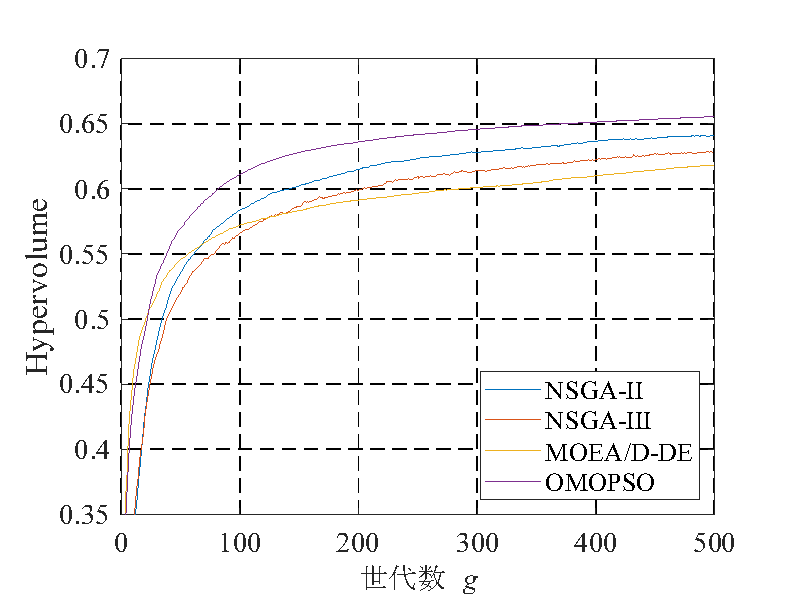
\includegraphics[width=0.7\linewidth]{fig/sim_result_hv_multi.eps}
  \end{center}
  \caption{4種類の多目的進化計算法による探索性能(Hypervolume値)の世代推移}
  \vspace{-6mm}
  \label{fig::sim_result_hv_multi}
\end{figure}

\begin{figure}[htbp]
  \begin{center}
    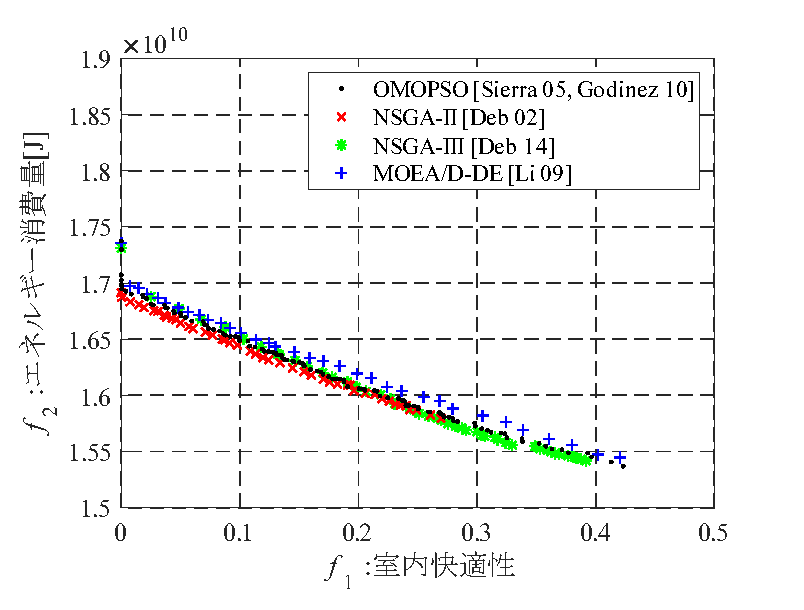
\includegraphics[width=0.7\linewidth]{fig/sim_result_pareto_multi.eps}
  \end{center}
  \caption{4種類の多目的進化計算法により獲得したパレートフロントの例}
  \vspace{-6mm}
  \label{fig::sim_result_pareto_multi}
\end{figure}

\red{
  4種類の手法でそれぞれ獲得した解集合の各世代のHVの平均値を\figref{fig::sim_result_hv_multi}に示す.本最適化問題においては,いずれの手法でも探索初期の35世代目までに実行可能解を発見することができ,その後HV値の高い良好な解の探索が進行した.最終世代では,4手法のうちOMOPSOが最も良いHVを示し,次いでNSGA-II, NSGA-III, MOEA/D-DEの順であった.MOEA/D-DEは探索初期の25世代程度は良い解を探索できているものの,その後の探索の進行が遅く,最終世代では最も悪いHV値となった.
  続いて,20回の試行のうち1回目の試行における,4種類の方法の最終世代に得られた解集合の例を\figref{fig::sim_result_pareto_multi}に示す.
}
最終世代では,いずれのアルゴリズムを用いても制約を満たし室内快適性とエネルギー消費量のトレードオフを表すスケジュール集合が獲得できていることがわかる.室内快適性$f_1$が0~0.2の範囲ではNSGA-II,0.2以上の範囲ではNSGA-IIIが,他の方法より良好な解集合を獲得したことがわかる.一方,OMOPSOは,室内快適性とエネルギー消費量のトレードオフを最も広範囲に表現する解集合を獲得したことがわかる.一方,MOEA/D-DEによる解集合は,目的関数空間の広域に分布するものの,他の方法による解集合と比較してパレートフロントに対する収束性が低いことがわかる.

\red{
  ここで,NSGA-II,NSGA-III,MOEA/D-DEが,OMOPSOに対して良好なHV値を獲得できなかった理由を考察する.
  まず,\figref{fig::sim_result_pareto_multi}のNSGA-III,MOEA/D-DEの分布を見ると,他の手法よりも解の間隔が広い事がわかる.これは,個体群の数が少ないことと,NSGA-IIIやMOEA/D-DEが用いる参照ベクトルの間隔が広く問題に対して偏りがあることが理由であると考えられる.このため均一で密度の高い解集合が獲得できておらず,高いHV値が得られていないものと考える.次に,NSGA-II,NSGA-IIIの解分布を見ると,他の手法に比べ$f_1$の快適性の値が大きい制約の境界に近い解が得られておらず,高いHV値の獲得が妨げられている.一方で,OMOPSOやMOEA/D-DEは,制約の境界付近の解を生成できており,広い分布の解が得られている.これは,NSGA-II,NSGA-IIIの解生成手法によるものと考える.OMOPSO,MOEA/D-DEでは,PSO・DEを用いた解生成を行っている.PSOは\subsecref{subsec::OMOPSO}に述べたように,個体群のうち良好な粒子方向のベクトルを足し合わせる交叉.DEはターゲットベクトルと変異ベクトルの交叉を用い,個体群の領域付近とその外側に確率的に子個体を生成する.一方,NSGA-II,NSGA-IIIで採用するSPXおよびPMは,\subsecref{subsec::ec}で述べたように,2つの親個体が持つ変数を中心とした各設計変数の周囲のみに子個体を生成するといった独特な解生成分布の特徴を持つ.このSBXとPMの持つ,生成される子個体の分布の特徴は,本問題の限られた領域の収束性の高い良好な解の発見には有効であったものの,制約付近の解の生成には有効ではなく,結果としてNSGA-II・NSGA-IIIは他手法のような広い範囲に分布する解集合の獲得ができなかったと考える.
}

\begin{comment}
\begin{table}[t]
  \begin{center}
    \caption{4種類の多目的進化計算法によるシミュレーション最適化で獲得した解集合のHypervolume(HV)値}
    \label{tab::sim_result_hv}
    \small
    \begin{tabular}{c|c|c|c|c}
      \hline
      手法 & NSGA-II & NSGA-III & MOEA/D-DE & OMOPSO \\
      \hline \hline
      HV値 & 0.621   & 0.628    & 0.589     & 0.643  \\
      \hline
    \end{tabular}
  \end{center}
\end{table}
\end{comment}

これらの結果から,提案システムで採用したOMOPSOは,他の多目的進化計算法と比較して高い性能を示し,室内快適性とエネルギー消費量のトレードオフを広域に近似可能で,ビル管理者に多様な設定温度スケジュール群を提示可能なアルゴリズムであるといえる.ただし,室内快適性が高い$f_1 \leq 0.2$の範囲ではNSGA-IIの性能が高いなど,提案システムにおける最適化アルゴリズムは代替可能であり,ビル管理者が求める性能によってアルゴリズムには選択の余地がある.

\subsection{OMOPSOによるアルゴリズム上の工夫の効果}
\subsubsection{目的}
本論文の提案システムにおいて,通常のMOPSOではなくOMOPSOを採用する意義について検証する.OMOPSOには\subsecref{subsec::OMOPSO}に記載したとおり,$\epsilon$-アーカイブという$\epsilon$優越でランク1となる解をサイズ制限無しに格納するアーカイブ,粒子の飛翔に用いるリーダー粒子群,一様突然変異・非一様突然変異・突然変異なしという3種の操作を加える突然変異,といったアルゴリズム上の工夫が行われている.これらの工夫はそれぞれ通常のMOPSOに対して解探索性能の向上を目的として導入したものであるが,これらの工夫が空調設定スケジュール最適化に対して有効でなければ,その工夫は必ずしも必要でないことになる.本項では,OMOPSOに対してこれらの工夫をそれぞれ無効化したアルゴリズムによって得られた解集合のHVを比較することで,提案システムにおいてOMOPSOを採用する意義と効果を明らかにする.

\subsubsection{方法}
OMOPSOを方法1, OMOPSOの工夫をそれぞれ無効化したアルゴリズム(方法2~4)を\tabref{tab::sim_cond_omopso_algo}の様に3つ定める.方法2は,$\epsilon$-アーカイブに対して最大アーカイブサイズを導入し,アーカイブサイズを超過する場合は混雑距離の短い解を除去する方法である.方法3は,リーダー粒子群を用いず,飛翔の際は$\epsilon$-アーカイブからバイナリトーナメントで選択した解をgBestとして用いる方法である.方法4は,突然変異を用いず,飛翔した粒子群をそのまま次世代の粒子群として用いる方法である.これらのアルゴリズムで空調設定スケジュール最適化を試行した結果を比較する.方法1~4は,ともに\tabref{tab::sim_param_omopso}に示すパラメータを用いる.ただし,方法2ではアーカイブサイズは100とする.また,本実験では,それぞれの方法1~4について初期値のシードを変更して20回の試行を行い,その平均のHVを比較する.

\begin{table}[ht]
  {\small
    \begin{center}
      \caption{OMOPSOのアルゴリズム上の工夫の検証方法}
      \label{tab::sim_cond_omopso_algo}
      \begin{tabular}{c|c|c|c|c}
        \hline
        方法  & 条件                 & アーカイブサイズ & リーダー粒子群 & 突然変異        \\
        \hline \hline
        方法1 & 通常のOMOPSO         & 制限なし         & あり           & 3種突然変異操作 \\
        方法2 & アーカイブサイズ制限 & 制限あり         & あり           & 3種突然変異操作 \\
        方法3 & リーダー粒子群不使用 & 制限なし         & なし           & 3種突然変異操作 \\
        方法4 & 突然変異なし         & 制限なし         & あり           & なし            \\
        \hline
      \end{tabular}
    \end{center}
  }
\end{table}

\subsubsection{結果}
20回試行によって得られた各世代の解集合のHVの平均値の推移を\figref{fig::sim_result_omopso_hv}に示す.本結果から,100世代までの探索初期では,方法2・方法4のアーカイブサイズに制限を設けた手法および突然変異操作を行わない手法が良いHV値を示すが,探索後期になると方法2, 方法3,方法4のHV値は方法1の通常のOMOPSO手法に劣った値を示すことがわかる.また,最終世代の解集合のHVの平均値を\tabref{tab::sim_result_omopso_hv}に示す.最終世代では方法1の通常のOMOPSOのHV値が他の方法のHV値よりも大きくなった.これらの結果から,方法2, 3, 4で示した,サイズ無制限の$\epsilon$-アーカイブ導入,リーダー粒子群を使用した飛翔,3種類の突然変異操作といった工夫が,本論文で取り上げた空調設定スケジュール最適化問題に対するOMOPSOの探索性能の向上に寄与していることが示された.
方法2,4が探索初期に良好な結果を示したのは,無制限のアーカイブサイズや突然変異操作がより多様な解探索を促進する手法であり,解集合の多様性よりもパレートフロントへの収束性が求められる探索初期には,これらの手法を含まないアルゴリズムのほうが早期に良好な解集合を探索できていたことが原因であると考えられる.ここから,OMOPSOのさらなる探索性能向上の工夫として,探索初期は$\epsilon$-アーカイブのサイズ制限を設けたり突然変異を行わずに探索し,ある解集合の分布が得られた段階でアーカイブサイズを拡張したり突然変異操作を行い,より多様な解の探索に切り替える手法が有効であると示唆される.


\begin{figure}[htbp]
  \begin{center}
    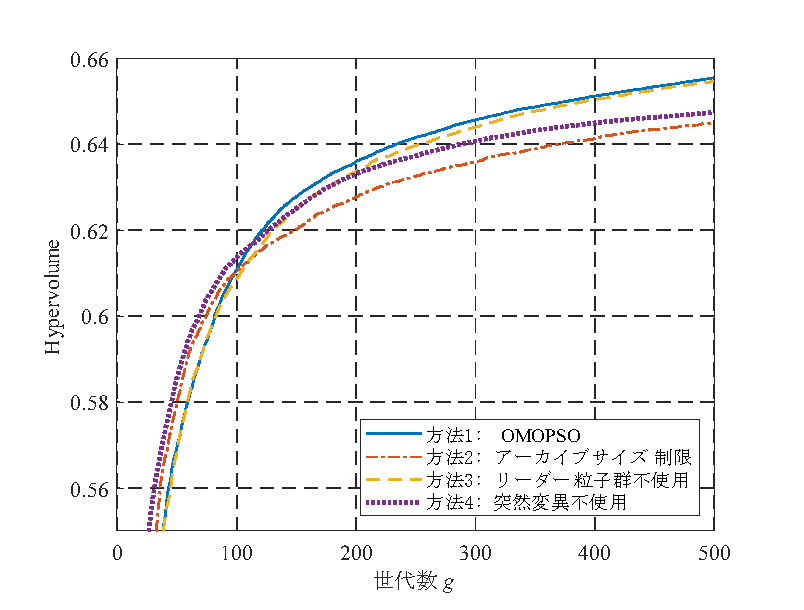
\includegraphics[width=0.7\linewidth]{fig/sim_result_omopso_hv.eps}
  \end{center}
  \caption{OMOPSOのアルゴリズム上の工夫によるHV値の世代推移の比較}
  \vspace{-6mm}
  \label{fig::sim_result_omopso_hv}
\end{figure}

\begin{table}[ht]
  {\small
    \begin{center}
      \caption{OMOPSOのアルゴリズム上の工夫によるHV値の比較}
      \label{tab::sim_result_omopso_hv}
      \begin{tabular}{c|c|c}
        \hline
        方法  & 条件                 & HV値   \\
        \hline \hline
        方法1 & 通常のOMOPSO         & 0.6554 \\
        方法2 & アーカイブサイズ制限 & 0.6546 \\
        方法3 & リーダー粒子群不使用 & 0.6474 \\
        方法4 & 突然変異なし         & 0.6451 \\
        \hline
      \end{tabular}
    \end{center}
  }
\end{table}


\section{結言}
本章では,オフィスビル全体の空調設定スケジュールを,シミュレーションを用いて最適化する手段について述べた.提案したシステムは,建築分野で用いられるシミュレータであるEnergyPlusを用いたシミュレーションにより,目的関数および制約を計算する.シミュレータに対してOMOPSOアルゴリズムを適用して,空調設定スケジュールの非劣解集合を探索した.実験結果により室内快適性とエネルギー消費量の双方が良好なスケジュールの非劣解集合を獲得できることを示した.
また,本研究で導入した制約条件が,快適性の良好なスケジュール獲得に寄与することを示した.さらに,$\epsilon$制約法をPSOとDEに組み込んだ単一目的最適化手法より,多目的最適化する手法のほうが良好なスケジュールを獲得できることを示した.加えて,代表的な多目的最適化手法であるNSGA-II,NSGA-III,MOEA/D-DEと比較して,OMOPSOは,最も広範囲に広がり,良好なHypervolume値を示す非劣解集合を獲得できることを示した.そして,OMOPSOが従来のMOPSOに対して持つアルゴリズム上の工夫が,本シミュレーション最適化の探索性能向上に寄与していることを示した.
本章で述べた試みにより,ビル全体の空調設定スケジュール最適化のために,シミュレーションを利用する方法の実現可能性が示された.

一方で,シミュレーションに基づく最適化には時間がかかる.1つのスケジュールの評価に約40秒かかり,一日の設定温度スケジュールを得るための最適化の全工程には約37.5時間かかる.これが原因となり,2つの問題が生じる.

1つ目は,精度の低い気象予報が最適化に悪影響を与えることである.シミュレータには,外気温予報を$\mathcal{A}$として入力する.予報と実際には差異が生じるが,直近の予報ほど正確性が高い\cite{JMA19}.本章の最適化システムは,最適化に約37.5時間かかるため,空調の運転を開始する一日半前の外気温予報を利用せざるを得ない.予報と実際の気象に差異が生じると,得られた空調設定スケジュールが最適にならないリスクがある.外気温の予報と実際の差異を考慮できれば,この問題を軽減できる可能性がある.この問題には,次の\chapref{chap::robust}で述べるロバスト最適化法で対処する.

2つ目は,進化計算で最適化するために十分な評価回数を実行できない恐れがあることである.進化計算は,膨大な解を生成しながら解評価をもとに探索を行い最適化する.1つの解の評価に時間がかかる場合,総評価回数を少なくせざるを得ず,最適化結果に影響を与える.この問題への対処法としてEnergyPlusのシミュレータの出力をもとに,エネルギー消費量・室内快適性のみを簡易に推定することで進化計算を加速するサロゲート最適化がある.本手法は,\chapref{chap::surrogate}で詳しく述べる.
